\documentclass[conference]{IEEEtran}
\IEEEoverridecommandlockouts

% --- Encoding and fonts ---
\usepackage[T1]{fontenc}
\usepackage[utf8]{inputenc}

% --- Layout ---
\usepackage{microtype}

% --- Math ---
\usepackage{amsmath}
\usepackage{amssymb}
\usepackage{amsfonts}

% --- Figures and tables ---
\usepackage{graphicx}
\graphicspath{{figures/}}
\usepackage{array}
\usepackage{tabularx}
\usepackage{booktabs}
\usepackage{pgfplots}
\pgfplotsset{compat=1.18}
\usepackage{stfloats}
\usepackage{placeins}
\usepackage{float}
\usepackage{textcomp}
\usepackage{xcolor}

% --- Bibliography ---
\usepackage[backend=biber,style=ieee,sorting=none]{biblatex}
\addbibresource{bibliography.bib}
\renewcommand*{\bibfont}{\footnotesize}

% --- Links ---
\usepackage{xurl}
\usepackage[hidelinks]{hyperref}
\usepackage{cleveref}

\newcolumntype{L}{>{\raggedright\arraybackslash}X}

% Wide tables/figures use the full page width (table*/figure*).
% Allow several of them on one page so leftover floats do not sit
% alone on an almost-empty sheet.
\setlength{\dblfloatsep}{8pt plus 2pt minus 2pt}
\setlength{\dbltextfloatsep}{8pt plus 2pt minus 2pt}
\setcounter{topnumber}{4}
\setcounter{dbltopnumber}{4}
\setcounter{totalnumber}{6}
\renewcommand{\topfraction}{0.95}
\renewcommand{\dbltopfraction}{0.95}
\renewcommand{\textfraction}{0.05}
\renewcommand{\floatpagefraction}{0.7}
\renewcommand{\dblfloatpagefraction}{0.7}
\raggedbottom

% Pack float-only pages from the top instead of stretching two
% wide tables apart with a large empty band.
\makeatletter
\setlength{\@fptop}{0pt}
\setlength{\@fpsep}{8pt plus 1pt minus 1pt}
\setlength{\@fpbot}{0pt plus 1fil}
\setlength{\@dblfptop}{0pt}
\setlength{\@dblfpsep}{8pt plus 1pt minus 1pt}
\setlength{\@dblfpbot}{0pt plus 1fil}
\makeatother

\pgfplotsset{
  ieee stacked bars/.style={
    ybar stacked,
    ymin=0,
    ymax=100,
    width=\linewidth,
    height=4.0cm,
    enlarge x limits=0.14,
    ylabel={Testable comparisons (\%)},
    ylabel style={font=\small},
    xtick=data,
    axis on top,
    ymajorgrids=true,
    grid style={gray!25},
    tick label style={font=\scriptsize},
    x tick label style={
      font=\scriptsize,
      align=center,
      text width=2.05cm,
    },
    legend style={
      at={(0.5,-0.28)},
      anchor=north,
      legend columns=4,
      font=\scriptsize,
      draw=black!45,
      /tikz/every even column/.append style={column sep=10pt},
    },
    legend cell align=left,
  }
}

\begin{document}

\title{Custom Memory Allocator Profiling}

\author{%
\IEEEauthorblockN{Jacob Nance}
\and
\IEEEauthorblockN{Fernanda Gonzalez}
\and
\IEEEauthorblockN{Francisco Chagua}
\and
\IEEEauthorblockN{Nicholas Hooper}
\and
\IEEEauthorblockN{Nicholas Johnson}
\and
\IEEEauthorblockN{Mohamed Konsowa}
}

\maketitle

\section*{Abstract}

Custom memory allocators can improve performance through control over memory
layout and aiding access patterns, but the benefit is largely dependent on the use
case. This paper profiles eight versions of a custom memory allocator against
regular global new across four workload pairs. The pairs are matrix array,
uniform matrix nodes, nested matrix stress, and linked list. The versions progress by
addressing fragmentation, coalescing of free memory blocks, allocation search
cost, and lock contention. Progression culminates with a proposed design
specialized for optimizing memory access patterns for matrix arithmetic operations.
Each pair was ran at three time scales on several machines and
operating systems, and a threaded matrix workload was examined as well.
Elapsed time, peak memory, page faults, and context switches were
recorded across repeated runs using matching arguments, seeds, and build
settings.

\section{Introduction and Research Questions}
\label{sec:introduction}

Regular global \texttt{new} was compared with eight versions of a custom
allocator.
The custom allocator requested one large region of memory from the operating
system and then handed out pieces from that region.
Each workload was built twice from the same source, with one
one using the built-in \texttt{new} and \texttt{delete}, and 
the other redirecting every allocation in the program into the custom memory pool.

The four workload pairs profiled were matrix array, uniform matrix nodes,
nested matrix stress, and linked list.
Each pair was run at three lengths, from a few minutes to more than six hours.
Runs were made on several machines and operating systems using matching
arguments, seeds, and build settings, with the results kept separate.
Elapsed time was recorded for every run.
Peak memory, page faults, and context switches were recorded where the
profiling tools reported them.
No single workload or machine was treated as evidence that one allocator is
always faster than another.

The investigation and analysis of this project addressed four main questions:

\begin{itemize}
  \item How did each version track free memory, select a free block, split and reuse
    blocks, recombine neighboring blocks, align allocations, and account for
    metadata?
  \item What advantages and costs did those choices carry for fragmentation,
    allocation search cost, and lock contention?
  \item What did specializing a version for matrix arithmetic trade away on
    other allocation patterns?
  \item Could a simpler multi-threaded implementation be made competitive by
    pairing it with the custom allocator?
\end{itemize}


\section{Background}
\label{sec:background}

In the C++ language, a program that calls \texttt{new} first asks an allocator for a block of free memory.
The allocator then finds a free block large enough, records that the block is in
use, and returns a pointer to it.
\texttt{delete} will then return the block back so it can be used again.
The base allocator supplied with the operating system serves every program on the
machine, so it is built for the average case rather than for any one memory access
pattern.
Performance costs related to memory allocation can come from searching for a block that fits, from locking shared
structures so that threads do not corrupt them, from the gaps left between
blocks as memory is reused, and from the work the operating system does to
supply memory as a program grows.
Searching longer for a tighter fit wastes less space but takes more time, and
holding more free memory in reserve avoids requests to the operating system at
the cost of a larger footprint.
When the memory access pattern of a program is known, opting for a custom memory allocator
can improve performance by tuning the structure and algorithm of allocation to fit it. 

\section{Explanation of Allocator Versions}
\label{sec:allocator-versions}

The custom allocator was changed in seven tagged versions.
Each tagged version replaces the previous implementation.
Table~\ref{tab:allocator-versions} records what each version does and what changed from the version immediately before it.

\begin{table}[htbp]
\centering
\small
\begin{tabularx}{\textwidth}{@{}l L L@{}}
\toprule
Version & Behavior & Change from previous \\
\midrule
v1 & One ordered free list, first-fit allocation, and immediate merging of adjacent free blocks. & Baseline. \\
v2 & Replaces first-fit with best-fit, selecting the smallest suitable free block. & Search policy on the free list changes from first-fit to best-fit. \\
v3 & Organizes free blocks into size-segregated lists. & The single free-list organization is replaced by size-segregated lists. \\
v4 & Adds fixed thread-local caches for small allocations. & Fixed thread-local caches are added for small allocations. \\
v5 & Defers merging adjacent free blocks until an allocation cannot otherwise be satisfied. & Adjacent free blocks are no longer merged immediately. \\
v6 & Adds batch cache refills and reusable small-block slabs. & Cache refills are batched and reusable small-block slabs are added. \\
v7 & Makes cache limits adaptive by growing frequently used size classes while retaining the overall cache-memory limit. & Cache limits become adaptive for frequently used size classes; the overall cache-memory limit is retained. \\
\bottomrule
\end{tabularx}
\caption{Custom allocator versions v1--v7 and the change introduced by each tag.}
\label{tab:allocator-versions}
\end{table}

\section{Experimental Methodology}
\label{sec:methodology}

\subsection{Data Collection}
The methodology for the data collection in this project was to split the data collection between groups. Each group was assigned 2-3 allocator versions to test, along with each team testing their own version 8.0.0 of the custom memory allocator.
To simplify the testing process, Group 2 created bash scripts for each workload to run the short, medium, and long runs for a specified version. This allowed each version to be tested on the same environment so that the results can be accurately compared for regular vs overloaded runs. 
However, this creates a limitation when comparing results between versions so the data analysis is more focused on the regular vs overloaded runs.

When collecting the data, the gnu time command was used to collect the runtime, memory usage, CPU usage, Voluntary Context Switches, Involuntary Context Switches, Minor Faults, and Major Faults for each run. The data was then collected into a CSV file for analysis. Each run was repeated 5 times to ensure that the results were consistent and to account for any variability in the system.
The data was then shared over Discord to a shared Excel file for comparison. This file consists of tables where each team can input their data.

\subsection{Data Analysis}
When performing the data analysis, an ANOVA test and Chi-Squared test were performed to determine if there is any statistically significant difference between the regular memory allocation and the custom allocator versions. 
Another comparison was made between the test results between teams of the same allocator version and workload. Although the data was not confirmed to have the same parameters, the comparison was still made to show a basic comparison on whether the different environments have significant differences in the results.
An additional ANOVA test was performed on all of the additional metrics collected by gnu time to determine what are significant contributors to the runtime differences between the regular memory allocation and the custom allocator versions.

\subsection{V8.0.0 Priorities}
When creating version 8.0.0 of the custom memory allocator, the team prioritized improving the performance of the allocator on the matrix workload. Additional details on the design process and decisions are in Section \ref{sec:improved-design}. 
\section{Hardware and Software Environments}
\label{sec:environments}

Two machines appear in the recorded files.
All Apple~M3~Max rows are the same Mac.
CSV \texttt{machine\_id} values that begin with \texttt{mohamed-m3max-} are campaign labels for that Mac, not separate computers.
The second machine is the Ryzen host used for v7 (\texttt{ryzen7900x-32gb-wsl}).

All recorded rows use project commit \texttt{12617e0f943a7b68d8334aa5477dfa403a75ca21}.

\subsection{Machines}

\begin{table}[H]
\centering
\caption{The two machines used in the supplied run files.}
\label{tab:machines}
\footnotesize
\begin{tabularx}{\textwidth}{@{}l L L@{}}
\toprule
Field & Apple M3 Max & AMD Ryzen 9 7900X \\
\midrule
Processor & Apple M3 Max & AMD Ryzen 9 7900X 12-Core Processor \\
Architecture & arm64 (v6 \texttt{environment.txt} field \texttt{architecture=arm64}) & x86\_64 (no architecture field in v7 \texttt{environment.txt}; library path \path{/usr/lib/x86_64-linux-gnu}) \\
OS & macOS, version depends on campaign (Table~\ref{tab:macos-campaigns}) & Windows 11 Home 10.0.26200; WSL 2.7.13.0; Ubuntu 24.04 LTS \\
Memory & 48~GB unified memory (v6 hardware addendum; per-batch core and memory fields were blank) & 32~GB DDR5-5200 host RAM; WSL \texttt{memory=24GB}, \texttt{swap=8GB} \\
Cores & 16 total (12 performance, 4 efficiency) & 12 physical / 24 logical \\
Compiler & Apple clang 17.0.0 (\texttt{clang-1700.6.3.2}) & Ubuntu \texttt{c++} 13.3.0 \\
Used for & matrix v1--v7 (all scales); v6 four-workload campaign & v7 four-workload campaign \\
\bottomrule
\end{tabularx}
\end{table}

\begin{table}[H]
\centering
\caption{macOS versions recorded on the Apple M3 Max, by campaign.}
\label{tab:macos-campaigns}
\footnotesize
\setlength{\tabcolsep}{8pt}
\begin{tabular}{@{}llll@{}}
\toprule
Campaign & Scale(s) & macOS version & OS build \\
\midrule
matrix v1--v7 & short, medium & 27.0   & 26A428 \\
matrix v1--v7 & long          & 26.6.2 & 25G83  \\
v6 four-workload & short, medium, long & 26.5.2 & 25F84 \\
\bottomrule
\end{tabular}
\end{table}

\subsection{CSV field comparison}

The matrix CSV
\path{matrix-v1-v7-short-medium-long.csv}
includes \texttt{machine\_id}, \texttt{processor}, \texttt{os\_version}, \texttt{os\_build}, and \texttt{project\_commit}.
The combined CSV
\path{v6-v7-run-durations.csv}
includes \texttt{machine\_id} only.
Processor, OS, architecture, and memory for the combined CSV come from adjacent \texttt{environment.txt} files.

\begin{table}[H]
\centering
\caption{Environment-field differences between the two supplied CSVs.}
\label{tab:csv-field-diff}
\footnotesize
\begin{tabularx}{\textwidth}{@{}l L L@{}}
\toprule
Field & Matrix CSV & Combined v6/v7 CSV \\
\midrule
\texttt{machine\_id} & yes (campaign labels; all M3 Max rows are the same Mac) & yes (M3 Max campaign label for v6; Ryzen label for v7) \\
\texttt{processor} & yes (Apple M3 Max) & no (adjacent \texttt{environment.txt}) \\
\texttt{os\_version} / \texttt{os\_build} & yes (Table~\ref{tab:macos-campaigns}) & no (adjacent \texttt{environment.txt}) \\
architecture & no column & no column \\
memory & no column & no column \\
\texttt{project\_commit} & yes (\texttt{12617e0f\ldots}) & no column (present in adjacent \texttt{environment.txt}) \\
\bottomrule
\end{tabularx}
\end{table}

For a list of all testing environments, listing the version and workload pairs along with the available machine and parameter information shared between teams at the time of data collection, see Tables~\ref{TestInventory1} and~\ref{TestInventory2} in Appendix~\ref{sec:appendices}.

\section{Workload Descriptions}
\label{sec:workloads}

UsingMatrixClass supplies four workload pairs.
Each pair is one shared header and two thin \texttt{main} wrappers.
The regular wrapper does nothing at start-up, so every \texttt{new} goes to
the C library.
The overloaded wrapper links the allocator's global \texttt{new} target.
It initializes the memory pool before the workload starts and shuts that pool
down after the workload ends.
Nothing else differs between the two programs of a pair.
The descriptions below are taken from the workload headers in the
UsingMatrixClass source tree.

\subsection{Properties shared by every workload}

\paragraph{Deterministic input.}
No workload reads the clock or the environment.
The matrix workloads fill matrices from a fixed deterministic generator, and
the linked list draws every decision from a generator with a fixed seed.
The regular and overloaded programs therefore execute the same sequence of
allocations, frees, and arithmetic.
Only the allocator differs.

\paragraph{Checksum.}
Every workload folds its results into a checksum and prints it on completion.
Matching checksums between the regular and overloaded runs prove that both did
the same work and that the overloaded allocator returned usable memory.
All 240 v6 and v7 runs and every M3~Max matrix row report matching checksums
(\Cref{sec:statistical-results}).

\paragraph{Pool sizing.}
The overloaded program has to tell the allocator how much memory to reserve
before the workload starts.
This is because the pool is one fixed \texttt{mmap} region that never grows.
Each workload computes that number from its own arguments.
The matrix workloads use the matrix size and count, the linked list uses its
maximum length, and the stress workload uses a fixed 512~MiB.
The regular program ignores the number.
One consequence matters when reading the results.
The overloaded program's peak memory reflects the pages it touched
inside that reservation, not the size of the reservation itself.

\paragraph{Single thread.}
Each workload program runs on one thread, and none of them creates additional
threads.
The allocator versions from v4 onward are built to be used by many threads at
once.
They add per-thread caches and lock-free ownership checks
(\Cref{sec:allocator-versions}).
However, the allocator does not create threads either.
In these experiments, therefore, the pool mutex is never contended and every
thread cache has exactly one owner.
What v4--v7 save here is the cost of the central bin search on a cache hit,
not time spent waiting for a lock.
The allocator's behavior under real concurrency is measured separately with
the multi-threaded matrix programs in \Cref{sec:pthreads-experiments}.

\subsection{Matrix array}

The matrix array workload lives in
\texttt{Matrix\allowbreak Array\allowbreak Workload.hpp}.
It creates 256 matrices of the same size $n$ and keeps them in one array for
the whole run.
The only command-line argument is the matrix size.
A matrix in MatrixClassDemo allocates each of its rows separately.
As a result, building one matrix costs $n$ allocations of about $8n$ bytes
each.

The program then runs 640 replacement passes.
During a pass, every matrix is replaced by a new matrix computed from the one
before it in the array.
Most of the time that computation is an addition.
For the 8 matrices whose index is a multiple of 32, it is a multiplication
instead.
Each computation produces a temporary result matrix, which is then copied into
the array slot and destroyed.
In other words, every pass allocates and frees 256 temporary matrices, and each
of those is $n$ row allocations.

The important thing about this workload is the balance between arithmetic and
allocation.
The allocations all have the same shape, so the allocator sees the same request
size over and over.
Meanwhile, the 8 multiplications in every pass each cost on the order of
$n^{3}$ floating-point operations, and they take up most of the run time.
It tests whether an overloaded allocator slows down a program that barely
needs it.
It is also the workload most sensitive to how rows are laid out in memory, which
is the reason the v8 redesign targeted it.

\subsection{Uniform matrix nodes}

The uniform nodes workload lives in
\texttt{Uniform\allowbreak Matrix\allowbreak Nodes.hpp}.
It also uses 256 matrices of one size $n$.
The difference is that each matrix is owned by its own separately allocated
node instead of sitting in a shared array.
The arguments are the matrix size and the number of replacement passes.

Each pass works the same way as the matrix array.
Every node is replaced by a new one computed from the node before it, using
addition most of the time and multiplication for every 32nd node.
However, replacing a node now means destroying the old node object and
allocating a brand new one to hold the result.
Because of that, the node's address changes on every pass, and each object
lives for only one pass rather than the whole run.

Since every matrix has the same size, the allocator sees only a few request
sizes.
These are the node object itself and the $n$ rows of its matrix.
Those sizes are requested and released constantly.
This is exactly the pattern that the v4--v7 thread cache and the v6--v7 slab
refills were designed for.
A block freed at one size is very likely to be requested again at that same
size a moment later.
Comparing this workload with the matrix array therefore isolates one thing.
The arithmetic is identical, so any difference between the two comes from the
added cost of destroying and recreating the node objects.

\subsection{Nested matrix stress}

The stress workload lives in
\texttt{Nested\allowbreak Matrix\allowbreak Stress.hpp}.
Instead of one flat array, it builds two trees of matrices.
There are six three-level trees (\texttt{Matrix***}) and four four-level trees
(\texttt{Matrix****}).
Each leaf of a tree holds between 6 and 18 matrices.
Unlike the other matrix workloads, the matrices here are not all the same
size.
Their dimensions are picked from twelve values ranging from 16 to 256.
That means row sizes range from 128 to 2048 bytes and whole matrices from
2~KiB to 512~KiB.
The only argument is a round count.

The leaf matrices are grouped in threes.
In each round, the program visits every group and stores the result of an
operation on the first two matrices into the third.
The operation is an addition most of the time and a multiplication every third
time.
Each operation allocates a fresh result matrix.
After the arithmetic, the round picks one outer branch of each tree at random,
destroys the whole branch, and rebuilds it with new random shapes.

This is the fragmentation workload.
Destroying a branch frees a large number of blocks of mixed sizes all at once.
The rebuild then immediately asks for a different mix of sizes.
That pattern puts pressure on the free-block data structure, which is a single
list in v1--v2 and size bins from v3 onward.
It also exercises the rule for splitting a block and returning the leftover.
Most of all, it separates the two coalescing policies.
Versions v1--v4 merge neighboring free blocks right away, while v5--v8 delay
merging until an allocation fails.
Finally, peak memory on this workload shows internal fragmentation.
The allocator rounds requests up to a 64-byte quantum, and most of the twelve
row sizes do not land on a quantum boundary, so some space is wasted in every
block.

\subsection{Linked list}

The linked list workload lives in
\texttt{Linked\allowbreak List\allowbreak Workload.hpp}.
It maintains a doubly linked list of \texttt{Node} objects.
A node is 72 bytes and holds two links, an index, a count, a pointer, six
integers, three characters, and four booleans.
Each node also owns a separately allocated array of 5 to 10 integers.
The only argument is the maximum list length, and the program performs 200
operations for every node of that maximum.

Every operation is chosen at random from a fixed mix.
Twenty percent of operations append a node.
Another twenty percent insert a node before a random existing node.
Twenty percent erase a random node.
Twenty-five percent update the fields of a random node without allocating.
The remaining fifteen percent replace a random node's integer array with a new
one of a different random length.
Once the list is full, append and insert turn into erase instead.
As a result, the list stays close to its maximum length for most of the run.

This workload is different from the other three because it does no matrix
arithmetic at all.
Each operation is a short pointer walk plus, in four of the five cases, one or
two allocations or frees of a few dozen bytes.
That makes it the pure allocator benchmark.
Run time is dominated by \texttt{new}, \texttt{delete}, and the cache misses
from touching millions of small objects scattered through memory.
It is also the workload where the allocator's own bookkeeping is proportionally
largest.
The header, back-pointer, and canaries described in
\Cref{sec:allocator-versions} add up to 64 bytes, which is almost as much as
the 72-byte node they are attached to.

\subsection{Run scales and parameter selection}

The assignment defines three run scales by how long they last.
Short runs take 3 to 5 minutes, medium runs take 2 to 3 hours, and long runs
take more than 6 hours.
Each scale requires five regular runs and five overloaded runs.
The parameters for each scale were chosen through calibration runs on each
machine, and those calibration runs do not count as measurements.
Because machines differ in speed, the same scale means different parameters on
different hosts.
\Cref{tab:workload-parameters} records the values that were run in every
campaign.

There were two different ways to make a run last longer, and they answer
different questions.

The first way is to repeat the same work.
The Group~2 campaigns on the Apple M3~Max and the Ryzen 7900X kept the program
arguments fixed and launched the executable several times in a row.
All of those launches were timed together as one run using
\texttt{repeat\allowbreak\_workload.sh}.
For example, a medium matrix run on the Ryzen host is \texttt{regular\_new 360}
launched 42 times in sequence, and a long run launches it 117 times.
In this approach the working set, the request sizes, and the pool size are the
same at every scale.
Only the number of repetitions changes.
As a result, these campaigns show almost no change in peak memory across
scales, and the gap between regular and overloaded \texttt{new} stays flat from
short to long.
One side effect is that start-up costs, such as the pool \texttt{mmap} and the
first-touch page faults, are paid once per repetition rather than once per
run.

The second way is to make the problem bigger.
The v2 campaign on the Core i7-1165G7 and the Group~1 campaigns launched each
executable once per measurement with a larger argument at each scale.
For example, the v2 matrix runs used sizes of 275, 800, and 1225, and the v2
linked list runs used maximum lengths of 125\,000, 580\,000, and 875\,000.
Here the working set grows along with the run time.
A larger matrix changes the row size and therefore the allocator's size class.
A longer list means more live blocks for a free-list search to walk through.
Peak memory grows as well.
This approach shows how an allocator responds to problem size.
However, a change from short to long cannot be blamed on duration alone.

These two approaches should not be compared with each other.
The flat scale behavior seen in the v6 and v7 campaigns should not be expected
in the v2 or Group~1 results.
Likewise, the very large v2 regressions on the stress and linked list
workloads at the long scale reflect a much bigger problem, not a longer clock.
\Cref{sec:statistical-results} keeps the two approaches in separate tables for
this reason.

\begin{table*}[!t]
\centering
\caption{Workload parameters that were run, by campaign. ``Reps'' is the
number of back-to-back executions timed as one run under the repeat strategy.
Values are from the campaign CSVs and \texttt{environment.txt} files; Group~1
values are from the shared data-collection sheet
(\Cref{sec:environments}). A dash means the scale was not run or not
recorded.}
\label{tab:workload-parameters}
\footnotesize
\setlength{\tabcolsep}{4pt}
\begin{tabularx}{\textwidth}{@{}l l l L L L l@{}}
\toprule
Campaign (host) & Versions & Workload & Short & Medium & Long & Strategy \\
\midrule
Group 2, Apple M3 Max & v1--v7 & Matrix array & 360, 1 rep & 360, 37 reps & 360, 97 reps & repeat (3 runs) \\
Group 2, Apple M3 Max & v6 & Matrix array & 360, 1 rep & 360, 37 reps & 360, 97 reps & repeat \\
 & & Uniform nodes & 350 700, 1 rep & 350 700, 37 reps & 350 700, 97 reps & repeat \\
 & & Nested stress & 800, 1 rep & 800, 34 reps & 800, 93 reps & repeat \\
 & & Linked list & 6\,500\,000, 1 rep & 6\,500\,000, 32 reps & 6\,500\,000, 84 reps & repeat \\
Group 2, Ryzen 9 7900X (WSL) & v7 & Matrix array & 360, 1 rep & 360, 42 reps & 360, 117 reps & repeat \\
 & & Uniform nodes & 350 700, 1 rep & 350 700, 42 reps & 350 700, 115 reps & repeat \\
 & & Nested stress & 800, 1 rep & 800, 38 reps & 800, 102 reps & repeat \\
 & & Linked list & 3\,512\,841, 1 rep & 3\,512\,841, 43 reps & 3\,512\,841, 120 reps & repeat \\
Group 2, Apple M3 Max & v8 & Matrix array & 360 & 360 & 360 & repeat \\
Group 2, Core i7-1165G7 (Ubuntu) & v2 & Matrix array & 275 & 800 & 1225 & grow \\
 & & Uniform nodes & 285 600 & 900 600 & 1200 600 & grow \\
 & & Nested stress & 100 & 440 & 900 & grow \\
 & & Linked list & 125\,000 & 580\,000 & 875\,000 & grow \\
Group 2, ThinkPad X13 (WSL) & v3 & Uniform nodes & 225 600 & 800 600 & -- & grow \\
 & & Nested stress & 200 & 1000 & -- & grow \\
Group 1, Ryzen 7 7800X3D (WSL2) & v4, v5 & Uniform nodes & 100 35\,000 & 100 1\,335\,000 & 100 4\,100\,000 & grow \\
Group 1, Apple M5 Pro & v4, v5 & Uniform nodes & 100 35\,000 & 100 1\,335\,000 & 100 4\,100\,000 & grow \\
Group 1, Core i5-6400 (Arch) & v5 & Matrix array & 400 & 900 & -- & grow \\
 & & Uniform nodes & 400 500 & -- & -- & grow \\
Group 1, Core i7-11800H & v5 & Matrix array & -- & -- & -- & not recorded \\
\bottomrule
\end{tabularx}
\end{table*}

\subsection{Expected sensitivity of each workload}

Reading the workload headers alongside the allocator versions in
\Cref{sec:allocator-versions} suggests where each pair should show a
difference and where it should not.
These expectations are written down here so that the results in
\Cref{sec:statistical-results,sec:charts-comparisons} can be judged against
them.

\begin{itemize}
  \item \textbf{Matrix array} should show the smallest effect of any version
    in either direction.
    The 8 matrix multiplications in each pass cost on the order of $n^{3}$
    operations each, and they swamp the 256 temporary-matrix allocations.
    Any difference that does appear is more likely to come from how rows are
    placed in memory than from allocation speed.
  \item \textbf{Uniform nodes} should reward versions that quickly reuse a
    freed block of the same size.
    That favors the v4--v7 thread cache and the v6--v7 slabs.
    It should penalize versions with an expensive free path, such as the
    v1--v2 address-ordered insertion with immediate merging.
  \item \textbf{Nested stress} should separate the two coalescing policies.
    Immediate merging in v1--v4 keeps large free spans available for the next
    rebuild.
    Deferred merging in v5--v8 makes each free cheap but risks a failed search
    followed by a full-region merge.
    This workload should also show the largest internal-fragmentation penalty
    in peak memory.
  \item \textbf{Linked list} should be the hardest workload for every custom
    version.
    The 64-byte header plus alignment and quantum rounding roughly triples the
    footprint of a 72-byte node.
    Meanwhile, the C library's small size classes and per-thread cache are
    already tuned for exactly this case.
\end{itemize}

Whether the measurements bear these expectations out is the subject of the
next two sections.

\section{Statistical Results}
\label{sec:statistical-results}

Values below are copied from the supplied CSVs.
Times are elapsed seconds.

\subsection{Matrix v1--v7}

Source: \path{matrix-v1-v7-short-medium-long.csv}.
Host: Apple M3 Max.
Workload is matrix, size 360.
Each row is 3 runs.
Concurrent processes in each batch: 6.
Checksum is consistent for every row: \texttt{4.8968250157139531e+119}.
All runs succeeded.
Repetitions: short $=1$, medium $=37$, long $=97$.
The column ``vs.\ regular (\%)'' is the CSV field \texttt{elapsed\_change\_vs\_regular\_percent}.
Rank is the CSV field \texttt{elapsed\_rank\_including\_regular} and includes Regular new.

\begin{table*}[!t]
\centering
\caption{Matrix short (360, 1 repetition), 3 runs. Times in seconds. Apple M3 Max, macOS 27.0.}
\label{tab:matrix-short}
\footnotesize
\setlength{\tabcolsep}{4pt}
\begin{tabular}{@{}l rrr rrr rr r@{}}
\toprule
Allocator & Run 1 & Run 2 & Run 3 & Mean & Median & Std.\ dev. & vs.\ regular (\%) & Rank \\
\midrule
Regular new & 247.20 & 247.32 & 247.18 & 247.233333 & 247.20 & 0.075719 & 0.000000 & 6 \\
v1.0.0 & 237.74 & 237.82 & 237.75 & 237.770000 & 237.75 & 0.043589 & $-3.827693$ & 1 \\
v2.0.0 & 237.85 & 237.85 & 237.87 & 237.856667 & 237.85 & 0.011547 & $-3.792639$ & 2 \\
v3.0.0 & 239.93 & 239.86 & 239.88 & 239.890000 & 239.88 & 0.036056 & $-2.970204$ & 3 \\
v4.0.0 & 241.05 & 241.01 & 241.03 & 241.030000 & 241.03 & 0.020000 & $-2.509101$ & 5 \\
v5.0.0 & 253.67 & 253.96 & 253.77 & 253.800000 & 253.77 & 0.147309 & 2.656060 & 8 \\
v6.0.0 & 240.35 & 240.23 & 240.24 & 240.273333 & 240.24 & 0.066583 & $-2.815154$ & 4 \\
v7.0.0 & 251.51 & 251.65 & 251.58 & 251.580000 & 251.58 & 0.070000 & 1.758123 & 7 \\
\bottomrule
\end{tabular}
\end{table*}

\begin{table*}[!t]
\centering
\caption{Matrix medium (360, 37 repetitions), 3 runs. Times in seconds. Apple M3 Max, macOS 27.0.}
\label{tab:matrix-medium}
\footnotesize
\setlength{\tabcolsep}{4pt}
\begin{tabular}{@{}l rrr rrr rr r@{}}
\toprule
Allocator & Run 1 & Run 2 & Run 3 & Mean & Median & Std.\ dev. & vs.\ regular (\%) & Rank \\
\midrule
Regular new & 9138.76 & 9138.39 & 9140.12 & 9139.090000 & 9138.76 & 0.910988 & 0.000000 & 6 \\
v1.0.0 & 8820.11 & 8821.59 & 8822.81 & 8821.503333 & 8821.59 & 1.352085 & $-3.475036$ & 2 \\
v2.0.0 & 8819.94 & 8819.70 & 8820.01 & 8819.883333 & 8819.94 & 0.162583 & $-3.492762$ & 1 \\
v3.0.0 & 8897.76 & 8901.31 & 8899.44 & 8899.503333 & 8899.44 & 1.775847 & $-2.621559$ & 3 \\
v4.0.0 & 8944.05 & 8944.77 & 8949.60 & 8946.140000 & 8944.77 & 3.017996 & $-2.111261$ & 5 \\
v5.0.0 & 9413.85 & 9411.98 & 9410.25 & 9412.026667 & 9411.98 & 1.800454 & 2.986475 & 8 \\
v6.0.0 & 8920.78 & 8920.32 & 8918.25 & 8919.783333 & 8920.32 & 1.347677 & $-2.399655$ & 4 \\
v7.0.0 & 9298.53 & 9298.39 & 9297.97 & 9298.296667 & 9298.39 & 0.291433 & 1.742041 & 7 \\
\bottomrule
\end{tabular}
\end{table*}

\begin{table*}[!t]
\centering
\caption{Matrix long (360, 97 repetitions), 3 runs. Times in seconds. Apple M3 Max, macOS 26.6.2.}
\label{tab:matrix-long}
\footnotesize
\setlength{\tabcolsep}{4pt}
\begin{tabular}{@{}l rrr rrr rr r@{}}
\toprule
Allocator & Run 1 & Run 2 & Run 3 & Mean & Median & Std.\ dev. & vs.\ regular (\%) & Rank \\
\midrule
Regular new & 24050.25 & 24048.46 & 24049.80 & 24049.503333 & 24049.80 & 0.931146 & 0.000000 & 6 \\
v1.0.0 & 23134.62 & 23135.86 & 23137.38 & 23135.953333 & 23135.86 & 1.382365 & $-3.798623$ & 1 \\
v2.0.0 & 23135.86 & 23137.51 & 23139.69 & 23137.686667 & 23137.51 & 1.921102 & $-3.791416$ & 2 \\
v3.0.0 & 23345.92 & 23345.17 & 23345.81 & 23345.633333 & 23345.81 & 0.405010 & $-2.926755$ & 3 \\
v4.0.0 & 23453.50 & 23453.57 & 23457.00 & 23454.690000 & 23453.57 & 2.000825 & $-2.473287$ & 5 \\
v5.0.0 & 24652.24 & 24648.64 & 24654.78 & 24651.886667 & 24652.24 & 3.085212 & 2.504764 & 8 \\
v6.0.0 & 23383.91 & 23384.51 & 23384.08 & 23384.166667 & 23384.08 & 0.309246 & $-2.766530$ & 4 \\
v7.0.0 & 24474.50 & 24477.54 & 24473.17 & 24475.070000 & 24474.50 & 2.240067 & 1.769545 & 7 \\
\bottomrule
\end{tabular}
\end{table*}

\subsection{v6 and v7 four-workload campaigns}

Source: \path{v6-v7-run-durations.csv}.
240 rows.
Five runs per (version, workload, scale, regular/overloaded) group.
Workloads: list, matrix, nodes, stress.
Scales: short, medium, long.
v6 ran on the Apple M3 Max.
v7 ran on the Ryzen 7900X WSL host.

\begin{table}[!ht]
\centering
\caption{v6.0.0 elapsed-time summary, 5 runs. Host: Apple M3 Max. Times in seconds.}
\label{tab:v6-means}
\scriptsize
\setlength{\tabcolsep}{3pt}
\begin{tabular}{@{}lllr r l@{}}
\toprule
Workload & Scale & Kind & $n$ & Mean (s) & Min--Max (s) \\
\midrule
list & short & regular & 5 & 276.5800 & 276.3400--276.8700 \\
list & short & overloaded & 5 & 277.3040 & 277.1200--277.5800 \\
list & medium & regular & 5 & 8810.2780 & 8807.1100--8814.0800 \\
list & medium & overloaded & 5 & 8832.6760 & 8830.7000--8835.1200 \\
list & long & regular & 5 & 23115.3800 & 23111.7500--23120.8500 \\
list & long & overloaded & 5 & 23161.0860 & 23159.1600--23163.6600 \\
matrix & short & regular & 5 & 248.0780 & 248.0400--248.1100 \\
matrix & short & overloaded & 5 & 242.1760 & 242.0800--242.3000 \\
matrix & medium & regular & 5 & 9156.1680 & 9155.4300--9157.8200 \\
matrix & medium & overloaded & 5 & 8943.7400 & 8942.2100--8945.0600 \\
matrix & long & regular & 5 & 24003.9360 & 24001.8900--24005.9500 \\
matrix & long & overloaded & 5 & 23445.8280 & 23443.2300--23448.4200 \\
nodes & short & regular & 5 & 248.6060 & 248.3700--249.4000 \\
nodes & short & overloaded & 5 & 240.9960 & 240.8900--241.1900 \\
nodes & medium & regular & 5 & 9173.6780 & 9168.4400--9177.8500 \\
nodes & medium & overloaded & 5 & 8893.1780 & 8891.0200--8895.7000 \\
nodes & long & regular & 5 & 24054.8500 & 24045.8500--24059.3300 \\
nodes & long & overloaded & 5 & 23320.3000 & 23318.0200--23323.9900 \\
stress & short & regular & 5 & 251.9720 & 251.8200--252.1800 \\
stress & short & overloaded & 5 & 269.6060 & 269.2500--269.8900 \\
stress & medium & regular & 5 & 8500.3520 & 8498.2700--8501.7300 \\
stress & medium & overloaded & 5 & 9038.6980 & 9035.1000--9041.0300 \\
stress & long & regular & 5 & 23317.4020 & 23225.6700--23417.2100 \\
stress & long & overloaded & 5 & 24683.3260 & 24679.3600--24686.2200 \\
\bottomrule
\end{tabular}
\end{table}

\begin{table}[!ht]
\centering
\caption{v7.0.0 elapsed-time summary, 5 runs. Host: AMD Ryzen 9 7900X (WSL). Times in seconds.}
\label{tab:v7-means}
\scriptsize
\setlength{\tabcolsep}{3pt}
\begin{tabular}{@{}lllr r l@{}}
\toprule
Workload & Scale & Kind & $n$ & Mean (s) & Min--Max (s) \\
\midrule
list & short & regular & 5 & 191.4180 & 189.5900--192.5100 \\
list & short & overloaded & 5 & 216.4060 & 214.8800--217.2200 \\
list & medium & regular & 5 & 8349.2000 & 8306.0000--8396.0000 \\
list & medium & overloaded & 5 & 9363.4000 & 9343.0000--9407.0000 \\
list & long & regular & 5 & 23348.6000 & 23290.0000--23427.0000 \\
list & long & overloaded & 5 & 25921.0000 & 25888.0000--25947.0000 \\
matrix & short & regular & 5 & 195.3200 & 193.8800--197.4900 \\
matrix & short & overloaded & 5 & 216.3020 & 213.8600--217.7800 \\
matrix & medium & regular & 5 & 8348.6000 & 8326.0000--8394.0000 \\
matrix & medium & overloaded & 5 & 9082.0000 & 9066.0000--9103.0000 \\
matrix & long & regular & 5 & 23198.6000 & 23170.0000--23234.0000 \\
matrix & long & overloaded & 5 & 25438.2000 & 25384.0000--25506.0000 \\
nodes & short & regular & 5 & 197.3820 & 196.2500--198.8400 \\
nodes & short & overloaded & 5 & 216.4000 & 214.6600--217.5800 \\
nodes & medium & regular & 5 & 8268.4000 & 8253.0000--8290.0000 \\
nodes & medium & overloaded & 5 & 9067.2000 & 9040.0000--9098.0000 \\
nodes & long & regular & 5 & 22537.8000 & 22524.0000--22560.0000 \\
nodes & long & overloaded & 5 & 24730.6000 & 24675.0000--24779.0000 \\
stress & short & regular & 5 & 219.4720 & 217.6200--221.6800 \\
stress & short & overloaded & 5 & 230.0680 & 228.2100--231.2300 \\
stress & medium & regular & 5 & 8368.0000 & 8339.0000--8398.0000 \\
stress & medium & overloaded & 5 & 8738.8000 & 8719.0000--8754.0000 \\
stress & long & regular & 5 & 22473.2000 & 22414.0000--22542.0000 \\
stress & long & overloaded & 5 & 23413.2000 & 23398.0000--23424.0000 \\
\bottomrule
\end{tabular}
\end{table}

\section{Charts and Comparisons}
\label{sec:charts-comparisons}

Figures~\ref{fig:runtime-outcomes} and~\ref{fig:metric-outcomes} summarize testable runtime and metric outcomes. The tables that follow report the environment ANOVA for several metric comparisons.
\subsection{Runtime by Data Structure}
\begin{figure}[H]
\centering
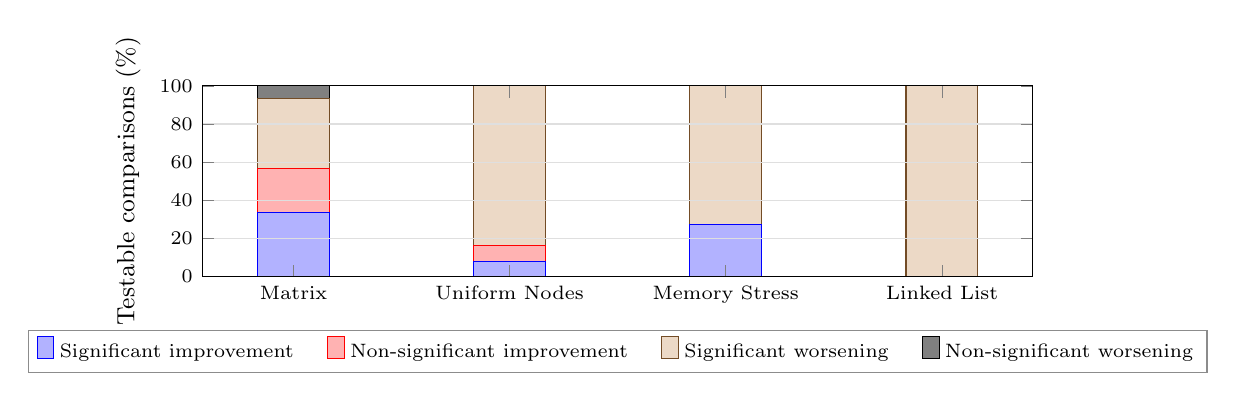
\begin{tikzpicture}
\begin{axis}[
  ieee stacked bars,
  bar width=26pt,
  xticklabels={Matrix, Uniform Nodes, Memory Stress, Linked List},
]
\addplot coordinates {(0,33.33333333) (1,8.00000000) (2,27.27272727) (3,0.00000000)};
\addlegendentry{Significant improvement}
\addplot coordinates {(0,23.33333333) (1,8.00000000) (2,0.00000000) (3,0.00000000)};
\addlegendentry{Non-significant improvement}
\addplot coordinates {(0,36.66666667) (1,84.00000000) (2,72.72727273) (3,100.00000000)};
\addlegendentry{Significant worsening}
\addplot coordinates {(0,6.66666667) (1,0.00000000) (2,0.00000000) (3,0.00000000)};
\addlegendentry{Non-significant worsening}
\end{axis}
\end{tikzpicture}
\caption{Runtime outcomes by data structure.}
\label{fig:runtime-outcomes}
\end{figure}

Figure~\ref{fig:runtime-outcomes} puts into perspective how effective the custom memory allocators are in improving the runtime of each of the workloads. 
Starting with the worst performance, the Linked Lists showed only significant worsening in all testing environments, run lengths, and allocator versions.
The Uniform Nodes workloads were second worst, with 84\% of the testable comparisons showing significant worsening, and 8\% showing non-significant improvement. Although it did improve in short and medium runs for version 3.0.0.
The Memory Stress workloads had about 27\% with significant improvement and the rest being significant worsening. Version 6.0.0 performed the best here as well, showing a consistent best showing from version 6.0.0.
Since the custom memory allocator is focused mainly on improving the performance of parallelized matrices, it had over 50\% improvement although about 20\% of that is non-significant.

\subsection{Metric Comparison}

\begin{figure}[H]
\centering
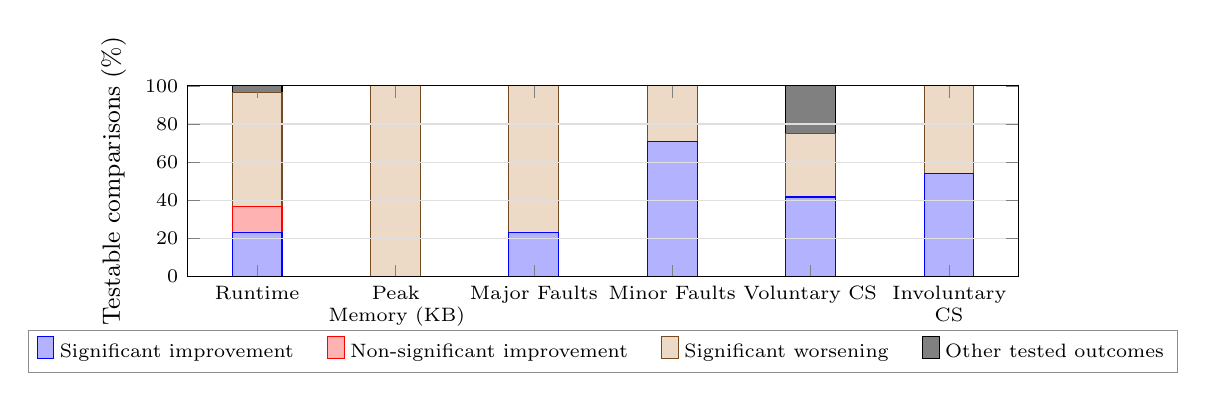
\begin{tikzpicture}
\begin{axis}[
  ieee stacked bars,
  bar width=18pt,
  enlarge x limits=0.10,
  x tick label style={font=\scriptsize, align=center, text width=1.7cm},
  xticklabels={Runtime, Peak Memory (KB), Major Faults, Minor Faults, Voluntary CS, Involuntary CS},
]
\addplot coordinates {(0,22.80701754) (1,0.00000000) (2,23.07692308) (3,70.83333333) (4,41.66666667) (5,54.16666667)};
\addlegendentry{Significant improvement}
\addplot coordinates {(0,14.03508772) (1,0.00000000) (2,0.00000000) (3,0.00000000) (4,0.00000000) (5,0.00000000)};
\addlegendentry{Non-significant improvement}
\addplot coordinates {(0,59.64912281) (1,100.00000000) (2,76.92307692) (3,29.16666667) (4,33.33333333) (5,45.83333333)};
\addlegendentry{Significant worsening}
\addplot coordinates {(0,3.50877193) (1,0.00000000) (2,0.00000000) (3,0.00000000) (4,25.00000000) (5,0.00000000)};
\addlegendentry{Other tested outcomes}
\end{axis}
\end{tikzpicture}
\caption{}
\label{fig:metric-outcomes}
\end{figure}

Figure~\ref{fig:metric-outcomes} focuses on additional measured metrics for the testing runs which focus on the weaknesses of certain workloads over each allocator. For example, the custom memory allocator always had a higher peak memory usage which only gets worse as the versions increased. This data however, is limited to team 2 tested versions 2, 7, and 8 although not enough data for a significance test was available with version 8.
One interesting metric from this is the difference between major and minor faults. While major faults increased significantly for the custom memory allocators, minor faults dropped up to 99+\% in version 7. However, for context switching, the custom memory allocator was better about preventing involuntary context switches while keeping it  about even in voluntary context switches.
In terms of runtime though, only about 20\% of runs had significant improvement.
For more data on the metrics see Table~\ref{PeakMemoryMetrics}, Table~\ref{MajorFaultsMetrics}, Table~\ref{MinorFaultsMetrics}, Table~\ref{VoluntaryContextSwitchMetrics}, and Table~\ref{InvoluntaryContextSwitchMetrics}.

\subsection{Environment Comparison Across Same Version and Workload}
The following table compares the same versions and workloads across multiple environments. However, this comes with the limitations that in order to reach the same run duration, the parameters may be different for some of these results.

\begin{table}[H]\caption{Environment ANOVA}
\centering\footnotesize\setlength{\tabcolsep}{5pt}\renewcommand{\arraystretch}{1.12}
\begin{tabular}{@{}llllcrrr@{}}
\toprule
Version & Workload & Comparison & Env.\ IDs & $n$ & $F$ & $p$ & Sig. \\ \midrule
v7.0.0 & Matrix & All Sizes & 1, 2 & 20 & 60.3979 & $3.6929\times10^{-7}$ & Yes \\
v7.0.0 & Matrix & Short & 1, 2 & 10 & 47.5496 & $1.2508\times10^{-4}$ & Yes \\
v6.0.0 & Matrix & All Sizes & 1, 2 & 20 & 374.4904 & $1.6999\times10^{-13}$ & Yes \\
v6.0.0 & Matrix & Short & 1, 2 & 10 & 111.9952 & $5.5525\times10^{-6}$ & Yes \\
v5.0.0 & Matrix & All Sizes & 1, 2 & 25 & 0.6923 & 0.4139 & No \\
v5.0.0 & Matrix & Short & 1, 2 & 10 & 0.5489 & 0.4799 & No \\
v5.0.0 & Matrix & Medium & 1, 2 & 10 & 0.4851 & 0.5058 & No \\
v5.0.0 & Uniform Nodes & All Sizes & 1, 2, 3 & 35 & 2,866.2357 & $8.1329\times10^{-37}$ & Yes \\
v5.0.0 & Uniform Nodes & Short & 1, 2, 3 & 15 & 874.0824 & $1.0041\times10^{-13}$ & Yes \\
v5.0.0 & Uniform Nodes & Medium & 1, 2 & 10 & 7,014.0642 & $4.6085\times10^{-13}$ & Yes \\
v5.0.0 & Uniform Nodes & Long & 1, 2 & 10 & 1,389.704 & $2.9414\times10^{-10}$ & Yes \\
v4.0.0 & Matrix & All Sizes & 1, 2 & 25 & 0.0879 & 0.7696 & No \\
v4.0.0 & Matrix & Short & 1, 2 & 10 & 35.7068 & $3.3235\times10^{-4}$ & Yes \\
v4.0.0 & Matrix & Medium & 1, 2 & 10 & 1.996 & 0.1954 & No \\
v4.0.0 & Uniform Nodes & All Sizes & 1, 2, 3 & 35 & 3,193.9375 & $1.4520\times10^{-37}$ & Yes \\
v4.0.0 & Uniform Nodes & Short & 1, 2, 3 & 15 & 1,376.1068 & $6.6936\times10^{-15}$ & Yes \\
v4.0.0 & Uniform Nodes & Medium & 1, 2 & 10 & 7,087.5386 & $4.4205\times10^{-13}$ & Yes \\
v4.0.0 & Uniform Nodes & Long & 1, 2 & 10 & 818.6869 & $2.4074\times10^{-9}$ & Yes \\
v3.0.0 & Matrix & All Sizes & 1, 2 & 15 & 1.452 & 0.2497 & No \\
v3.0.0 & Matrix & Short & 1, 2 & 10 & 4.1199 & 0.0769 & No \\
v2.0.0 & Matrix & All Sizes & 1, 2 & 20 & 4.6506 & 0.0448 & Yes \\
v2.0.0 & Matrix & Short & 1, 2 & 10 & 20.9244 & 0.0018 & Yes \\
\bottomrule\end{tabular}
\label{EnvAnova}
\end{table}

The key takeaways from Table~\ref{EnvAnova} are that all uniform nodes tests across environments had high levels of significance with p values much less than 10 to the 10th power. This means that there is a high likelyhood that the environment is playing a factor in the results.
However, the Matrix were split across the significance. This implies that across runs (mostly short and medium) there is little variation between systems which means that matrices are the better comparison metric when trying to determine across systems whether the custom memory allocator is effective or not.
\clearpage
\twocolumn
\section{Hardware and Operating System Discussion}
\label{sec:hardware-os-discussion}

The tested and referenced hardware used in this project includes the following:

\begin{itemize}
\item \textbf{Apple M3 Max, 48~GB unified memory, macOS, ARM64:} used for the
matrix v1--v7 campaign, the v6 four-workload campaign, and one v8 matrix group.
\item \textbf{MacBook Pro with Apple M2 Pro, 32~GB memory, macOS, ARM64:}
v8.0.0 development, integration and unit testing, custom metric analysis
\item \textbf{AMD Ryzen~9~7900X, 32~GB RAM, Ubuntu~24.04 under WSL, x86-64:}
used for the v7 four-workload suite.
\item \textbf{Intel i7-1165G7, 16~GB RAM, Ubuntu~24.04.3, x86-64:} used for
Jacob's v2 measurements and the newer v8 matrix runs.
\item \textbf{Intel i7-11370H, 16~GB RAM, WSL and Linux Mint, x86-64:} used for
the pthread comparison runs.
\item \textbf{Additional team systems:} newer Apple Silicon machines and other
Intel and Ryzen hosts appeared in the shared team inventory, although not all
of them contributed balanced measurements across allocator versions and
workloads.
\end{itemize}

These hardware differences matter because allocator behavior is tied closely to cache hierarchy, memory bandwidth,
scheduler behavior, and runtime overheads from the operating system environment. The Apple M3 Max results
represent an ARM64 macOS platform with high memory bandwidth and unified memory, while the Ryzen and
Intel hosts represent x86-64 Linux or WSL environments with different cache organizations, thread scheduling
behavior, and background-system costs. For that reason, environment should be treated as a source of
experimental variation rather than noise to be ignored. It cannot be assumed that a result that holds on one
machine will behave identically on every processor and operating system and should instead be interpreted with
the knowledge that the results may have been influenced by the machine they were run on.

\section{Improved Allocator Design}
\label{sec:improved-design}

\subsection{Design Goal}

The goal of v8.0.0 was not to completely replace the allocator policy introduced by v7.0.0, but to improve
the part of that design that too clumsy. In v7.0.0, the allocator already had segregated bins, thread-local
small-block caches, batch refill, deferred coalescing, and bounded retained cache memory. However, the problem
was that cache growth was still driven mainly by refill behavior. That policy could react to demand,
but it did so through an indirect signal.

The design goal in v8.0.0 was therefore to keep the same general architecture while changing how
the allocator decides which small-size classes deserve more cached capacity. Instead of treating repeated
refill events as the main indicator of importance, v8.0.0 measures live demand directly for exact reusable
slab sizes and uses that information to retune cache targets. This makes the allocator more workload-aware
without giving up the drop-in \texttt{new}/\texttt{delete} interface as they are part of the project's
deliverables. That direction is consistent with the broader motivation for custom allocators: once the
allocation pattern of a program is better understood, the allocator can be adapted to that pattern rather
than paying the full generality cost of a one-size-fits-all design~\cite{rakosCustomAllocators2021}.

\subsection{Baseline: What v7.0.0 Already Provided}

Version~7.0.0 inherited most of the important structural changes introduced between v3.0.0 and v6.0.0. Free
blocks were already grouped into segregated bins, which reduced the need to scan the entire heap for every
request. Small allocations could often be served from a thread-local cache, which reduced repeated global
locking on hot size classes. When those caches missed, the allocator could refill them in batches, gradually
decreasing the cost of central-pool access across several future allocations.

Version~7.0.0 no longer merged adjacent free blocks on every deallocation. Instead, it retained
the deferred-coalescing strategy from v5.0.0 and v6.0.0, so adjacent blocks were merged only when an allocation
request could not be satisfied directly. That design trades some fragmentation risk for lower steady-state
deallocation cost, a tradeoff that is common in dynamic allocation systems~\cite{wilson1995}. V7.0.0 also
limited retained cache bytes per thread, so cache growth was bounded even when a workload exercised the same
classes heavily.

These features matter because they define what V8.0.0 did \textit{not} need to change. The allocator already
had a practical free-structure layout, a central best-fit style search within bins, a cache for small hot
objects, and correctness machinery such as canaries and ownership checks. The main issue was not missing
functionality, but that one piece of policy, cache sizing, was still too blunt.

\subsection{Weakness in v7.0.0}

The weakness in v7.0.0 was that cache growth was based mostly on refill frequency. If a particular bin missed
repeatedly, the allocator interpreted that pattern as evidence that the class should keep more cached blocks.
That idea is sensible at a high level, but refill count is not the same thing as measured working-set demand.
A class can refill frequently because of a short burst, irregular reuse, or because the cached
capacity is briefly too small even though the long-term live set is modest.

This distinction matters because refill count is only an indirect signal. It tells the allocator that pressure
occurred, but not how many blocks were actually needed live at once. In practice, that means a hot phase can
leave a class overgrown after the workload shifts, while another class may deserve cached capacity for reasons
that are not well captured by miss events alone. The result overly reactive policy that might not be reacting
for the right reasons. V8.0.0 addresses exactly this problem by replacing refill-driven growth with measured
occupancy-driven retuning.

\subsection{High-Level V8.0.0 Strategy}

At a high level, V8.0.0 keeps the cache policy of V7.0.0. The allocator still uses segregated small and large
bins, still serves exact small slabs from a thread-local cache when possible, and still falls back to the
central pool on cache misses. But V8.0.0 adds explicit accounting for live exact-slab allocations and uses
that accounting to retune cache targets per size class.

The implementation also makes the allocator more observable. V8.0.0 introduces a metrics surface that records
cache hits, misses, searches, refills, flushes, tuning events, and mutex acquisitions. This does not directly
make the allocator faster, but it makes the allocator easier to analyze. That is a real design improvement in
the context of this assignment because elapsed time alone cannot explain why one workload improved while
another regressed.

\subsection{New Data Structures and Metrics}

The most visible interface addition in V8.0.0 is the \texttt{AllocatorMetrics} structure. It exposes counters
for thread-cache hits and misses, central-pool searches, searched free-list nodes, cache refills, cache
flushes, target-driven and byte-limit-driven flush events, coalescing on allocation failure, central mutex
acquisitions, and cache-policy tuning activity. Essentially turning the allocator into something that can
be measured rather than only timed.

The key internal addition is \texttt{CacheAccounting}. Each accounting record stores live-block counts for all
small-bin classes. When a thread cache is registered, it receives one of these accounting records and uses it
to track how many blocks of each exact slab size are live at the same time. Instead of inferring demand from
miss history, V8.0.0 can observe demand directly. The code also extends \texttt{ThreadCache} with per-bin arrays
for target sizes, peak live counts, and countdowns until the next tuning event.

Metrics are optionally enabled through a compile-time macro. That decision is important because profiling
counters are useful for analysis, but they can interfere with timing runs and skew data. The design therefore
separates observability from baseline execution cost.

\subsection{Exact Slab Classification}

Another important change in V8.0.0 is that the small-object cache is restricted to exact slab classes. The
helper \texttt{smallSlabSize} computes whether an allocation can be represented as one of these small exact
slab sizes after metadata, alignment, and quantum rounding are accounted for. If so, the allocator may serve it
from the thread cache; if not, the request follows the central-pool path.

This is more precise than treating every request below a broad threshold as interchangeable. Exact slab
classification means the cache is tuned around the actual reusable unit, not just the requested payload size.
That keeps the policy cleaner and reduces the chance that slightly different requests contaminate the same
reuse class. It also aligns naturally with the new accounting model, since occupancy is now tracked for the
slab sizes that the allocator truly reuses.

\subsection{Adaptive Cache Target Tuning}

Adaptive target tuning is the core improvement in V8.0.0. For each exact cached slab class, the allocator
tracks the current live count and the peak live count seen during a tuning window. After a fixed number of
allocations in that class, the allocator resets the cache target to a bounded function of observed demand:

\begin{equation}
\begin{aligned}
\text{new target} = {}& \operatorname{clamp}(\text{peak live blocks} + \text{cushion},\\
& \text{minimum},\ \text{maximum}).
\end{aligned}
\end{equation}

In the current implementation, the minimum cached target is eight blocks, the cushion is four blocks,
the retuning interval is 256 allocations in the class, and the maximum cached target is 512 blocks. This
policy is simple, but it is already more informative than refill-count doubling. A class grows because the
program actually kept that many blocks live, not only because a short miss burst happened to occur.

This retuning model still uses a heuristic, so it should not be described as optimal. However, it is a more
direct approximation to working-set size than the V7.0.0 rule. It also fits the broader principle that cache
effectiveness depends on matching capacity to the reuse pattern of the workload, not just reacting to misses
after the fact~\cite{hennessy2019}.

\subsection{Allocation and Deallocation Path Changes}

On the allocation path, V8.0.0 still begins by validating size and alignment and by registering the thread
cache if needed. If the request belongs to an exact small slab class, the allocator attempts a thread-cache
hit first. A successful hit no longer only returns a block; it also increments the accounting state through
\texttt{exactAllocationCounter}. If the request misses the thread cache, the allocator records the miss,
searches the central pool, and refills the thread cache when the request still belongs to an exact reusable
slab size.

The deallocation path was updated to mirror that model. When a block came from an exact cached slab class,
deallocation decrements the same live-count structure before the block is returned to the thread cache. This
is essential. Without deallocation-side accounting, the allocator could see when pressure rises, but not when
a class cools down. Updating both paths keeps the model synchronized with actual object lifetime.

Outside those changes, the general slow path remains familiar. Free-list insertion and removal still happen
in the central allocator, and coalescing still occurs only when allocation pressure requires it. That
continuity is useful because it isolates the effect of the new policy rather than mixing it with a wholesale
redesign of the free structure.

\subsection{What Stayed the Same}

Several important parts of the allocator did not change in v8.0.0. The allocator is still a singleton memory
pool behind global \texttt{new}, \texttt{new[]}, \texttt{delete}, and \texttt{delete[]}. It still uses
segregated small and large bins, retains a thread-local small-object cache, uses a central mutex for
global free-list work, and preserves canary-based corruption detection and ownership validation.

This continuity matters for interpretation. It means that v8.0.0 should not be described as an entirely new
allocator, and any measured behavior should not be attributed to a change in the whole allocation architecture.
Instead, the main change is a policy refinement inside an already established framework. That makes both the
design argument and the later experimental comparison cleaner.

\subsection{Why These Changes Were Chosen}

These changes were chosen for three practical reasons. First, they improve signal quality. Measured live
occupancy is closer to the true working set than refill count, so it is a better basis for deciding how much
cache capacity a class deserves. Second, they improve observability. By recording allocator events directly,
v8.0.0 makes it possible to explain results with evidence rather than only with conjecture. Third, they
preserve compatibility. The allocator remains reusable and fetchable by another project, and it still acts
as a drop-in replacement for the standard allocation interface.

There is also a pragmatic engineering reason for preferring this approach over a full rewrite. A focused
policy change is easier to validate, easier to compare against V7.0.0, and less likely to introduce unrelated
regressions. For this assignment, that is a better trade than introducing an entirely different
memory-management strategy and then trying to separate the effects afterward.

\subsection{Expected Effect on the UsingMatrixClass Workloads}

The expected effect of v8.0.0 depends on the workload. The matrix-array workload repeatedly creates and
replaces many objects with highly regular sizes. That regularity should give the exact-slab cache policy a
fair opportunity to discover stable hot classes and keep those classes warm. Uniform matrix nodes add more
lifetime churn, but still retain a relatively regular size pattern, so they should also benefit when live
occupancy remains concentrated in a narrow set of bins.

Nested matrix stress is a more mixed case. It uses several matrix sizes and repeatedly rebuilds subtrees, so
it exercises more classes and more transitions between them. This is a useful workload for testing whether
adaptive targets actually follow demand rather than simply inflating over time. The linked-list workload is
the most difficult case because it mixes many tiny nodes with additional dynamic arrays and highly active
updates. Even if v8.0.0 does not always improve this case, the policy is still motivated, since it should be
less likely than V7.0.0 to keep cold classes oversized after a burst.

The key point is that v8.0.0 was designed to improve policy quality, not to guarantee universal speedup. A
workload that benefits from stable exact slab reuse is a natural candidate for improvement. A workload
dominated by tiny-object metadata costs or central-pool behavior may still expose limitations.

\subsection{Validation and Test Support}

The repository includes tests that support both correctness and the new policy claims. The cache-focused
tests verify that reused small allocations can be served from the thread cache without forcing unnecessary
central-pool work. The cache-policy tests verify that the adaptive mechanism actually tunes targets and is
capable of both increasing and decreasing them over time. General memory-pool tests still cover best-fit reuse,
coalescing behavior, multithreaded use, and canary detection, while global allocation tests verify that the
allocator remains a correct replacement for ordinary \texttt{new} and \texttt{delete}.

This matters for the report because it shows that the improved design was not only described conceptually.
The design was implemented in a way that exposes measurable policy behavior and was tested at both the
allocator-core level and the integration level.

\subsection{Limitations}

V8.0.0 still has important limitations. The central free structure remains protected by one mutex, so global
allocator work is still serialized. Large allocations still depend on the same central allocator structure.
Metadata and canary checks remain present, which is useful for safety but still costs time and space. The
retuning policy itself is empirical and bounded by a few fixed constants, so it should be treated as a
practical heuristic rather than a theoretically optimal rule.

These limitations should be stated clearly because they define the scope of the contribution. V8.0.0
improves cache sizing and allocator observability. It does not eliminate all contention, all fragmentation
costs, or all workload-specific regressions.

\subsection{Summary}

Version~8.0.0 is best understood as a measured refinement of V7.0.0. It preserves the allocator family that
earlier versions built, but replaces refill-driven cache growth with occupancy-driven retuning for exact
reusable small slabs. At the same time, it introduces explicit metrics and accounting so allocator behavior
can be studied directly. The result is not a brand-new allocator architecture, but a more informed and more
analyzable one. That makes it a meaningful improvement for this project and a defensible basis for the
experimental comparisons in the next section.

\clearpage

\section{Improved Allocator Results}
\label{sec:improved-results}

\begin{figure}[H]\centering\begin{tikzpicture}\begin{groupplot}[group style={group size=3 by 2,horizontal sep=1.3cm,vertical sep=1.6cm},width=.29\textwidth,height=4.5cm,ymin=0,xmin=-.35,xmax=1.35,xtick={0,1},xticklabels={Regular,Overloaded},tick label style={font=\scriptsize},title style={font=\small},ylabel={Time (min)},ylabel style={font=\scriptsize}]
\nextgroupplot[title={Short, E1, $n=3$},ymax=4.879496666666666]
\addplot[gray!50,no marks] coordinates {(0,4.134833333333334) (1,3.9475)};
\addplot[gray!50,no marks] coordinates {(0,4.1339999999999995) (1,3.9478333333333335)};
\addplot[gray!50,no marks] coordinates {(0,4.135166666666667) (1,3.9481666666666664)};
\addplot[only marks,mark=*,mark size=1.8pt,color=blue!65!black] coordinates {(0,4.134833333333334) (0,4.1339999999999995) (0,4.135166666666667)};
\addplot[black,very thick,no marks] coordinates {(-0.12,4.134666666666667) (0.12,4.134666666666667)};
\addplot[only marks,mark=*,mark size=1.8pt,color=orange!80!black] coordinates {(1,3.9475) (1,3.9478333333333335) (1,3.9481666666666664)};
\addplot[black,very thick,no marks] coordinates {(0.88,3.947833333333333) (1.12,3.947833333333333)};
\nextgroupplot[title={Medium, E1, $n=3$},ymax=180.10379333333333]
\addplot[gray!50,no marks] coordinates {(0,152.60416666666666) (1,145.02466666666666)};
\addplot[gray!50,no marks] coordinates {(0,152.593) (1,145.02233333333334)};
\addplot[gray!50,no marks] coordinates {(0,152.63033333333334) (1,145.01383333333334)};
\addplot[only marks,mark=*,mark size=1.8pt,color=blue!65!black] coordinates {(0,152.60416666666666) (0,152.593) (0,152.63033333333334)};
\addplot[black,very thick,no marks] coordinates {(-0.12,152.60916666666665) (0.12,152.60916666666665)};
\addplot[only marks,mark=*,mark size=1.8pt,color=orange!80!black] coordinates {(1,145.02466666666666) (1,145.02233333333334) (1,145.01383333333334)};
\addplot[black,very thick,no marks] coordinates {(0.88,145.02027777777778) (1.12,145.02027777777778)};
\nextgroupplot[title={Long, E1, $n=3$},ymax=472.11701666666664]
\addplot[gray!50,no marks] coordinates {(0,400.0991666666667) (1,379.66299999999995)};
\addplot[gray!50,no marks] coordinates {(0,400.0315) (1,379.5996666666667)};
\addplot[gray!50,no marks] coordinates {(0,400.055) (1,379.61716666666666)};
\addplot[only marks,mark=*,mark size=1.8pt,color=blue!65!black] coordinates {(0,400.0991666666667) (0,400.0315) (0,400.055)};
\addplot[black,very thick,no marks] coordinates {(-0.12,400.0618888888889) (0.12,400.0618888888889)};
\addplot[only marks,mark=*,mark size=1.8pt,color=orange!80!black] coordinates {(1,379.66299999999995) (1,379.5996666666667) (1,379.61716666666666)};
\addplot[black,very thick,no marks] coordinates {(0.88,379.6266111111111) (1.12,379.6266111111111)};
\nextgroupplot[title={Short, E2, $n=5$},ymax=7.0192299999999985]
\addplot[gray!50,no marks] coordinates {(0,3.558666666666667) (1,4.843666666666667)};
\addplot[gray!50,no marks] coordinates {(0,3.5631666666666666) (1,5.133666666666667)};
\addplot[gray!50,no marks] coordinates {(0,4.285333333333333) (1,5.600666666666667)};
\addplot[gray!50,no marks] coordinates {(0,4.001) (1,5.948499999999999)};
\addplot[gray!50,no marks] coordinates {(0,4.045) (1,5.2091666666666665)};
\addplot[only marks,mark=*,mark size=1.8pt,color=blue!65!black] coordinates {(0,3.558666666666667) (0,3.5631666666666666) (0,4.285333333333333) (0,4.001) (0,4.045)};
\addplot[black,very thick,no marks] coordinates {(-0.12,3.8906333333333336) (0.12,3.8906333333333336)};
\addplot[only marks,mark=*,mark size=1.8pt,color=orange!80!black] coordinates {(1,4.843666666666667) (1,5.133666666666667) (1,5.600666666666667) (1,5.948499999999999) (1,5.2091666666666665)};
\addplot[black,very thick,no marks] coordinates {(0.88,5.347133333333334) (1.12,5.347133333333334)};
\nextgroupplot[title={Medium, E2, $n=5$},ymax=25.965899999999998]
\addplot[gray!50,no marks] coordinates {(0,16.54883333333333) (1,19.467499999999998)};
\addplot[gray!50,no marks] coordinates {(0,16.979499999999998) (1,20.186333333333334)};
\addplot[gray!50,no marks] coordinates {(0,17.910500000000003) (1,21.634999999999998)};
\addplot[gray!50,no marks] coordinates {(0,19.017999999999997) (1,21.90983333333333)};
\addplot[gray!50,no marks] coordinates {(0,17.458333333333332) (1,22.005)};
\addplot[only marks,mark=*,mark size=1.8pt,color=blue!65!black] coordinates {(0,16.54883333333333) (0,16.979499999999998) (0,17.910500000000003) (0,19.017999999999997) (0,17.458333333333332)};
\addplot[black,very thick,no marks] coordinates {(-0.12,17.583033333333333) (0.12,17.583033333333333)};
\addplot[only marks,mark=*,mark size=1.8pt,color=orange!80!black] coordinates {(1,19.467499999999998) (1,20.186333333333334) (1,21.634999999999998) (1,21.90983333333333) (1,22.005)};
\addplot[black,very thick,no marks] coordinates {(0.88,21.040733333333332) (1.12,21.040733333333332)};
\nextgroupplot[title={Long, E2, $n=5$},ymax=70.33999666666666]
\addplot[gray!50,no marks] coordinates {(0,59.61016666666667) (1,59.1565)};
\addplot[gray!50,no marks] coordinates {(0,56.32816666666667) (1,52.524833333333326)};
\addplot[gray!50,no marks] coordinates {(0,54.529833333333336) (1,53.0625)};
\addplot[gray!50,no marks] coordinates {(0,59.271499999999996) (1,50.753166666666665)};
\addplot[gray!50,no marks] coordinates {(0,57.594) (1,53.2515)};
\addplot[only marks,mark=*,mark size=1.8pt,color=blue!65!black] coordinates {(0,59.61016666666667) (0,56.32816666666667) (0,54.529833333333336) (0,59.271499999999996) (0,57.594)};
\addplot[black,very thick,no marks] coordinates {(-0.12,57.46673333333333) (0.12,57.46673333333333)};
\addplot[only marks,mark=*,mark size=1.8pt,color=orange!80!black] coordinates {(1,59.1565) (1,52.524833333333326) (1,53.0625) (1,50.753166666666665) (1,53.2515)};
\addplot[black,very thick,no marks] coordinates {(0.88,53.7497) (1.12,53.7497)};
\end{groupplot}\end{tikzpicture}\caption{V8 Matrix Array Regular versus Overloaded elapsed times. Dots are observations; lines connect presumed run pairs; black ticks are means. E1: mohamed-m3max-v8-full, $n=3$; E2: Jacob Nance v2 environment, $n=5$. Panels use separate zero-based time scales. Workloads differ across environments; Short/Medium/Long are within-group labels.}\label{fig:v8-paired}\end{figure}\clearpage
\begin{figure}[H]\centering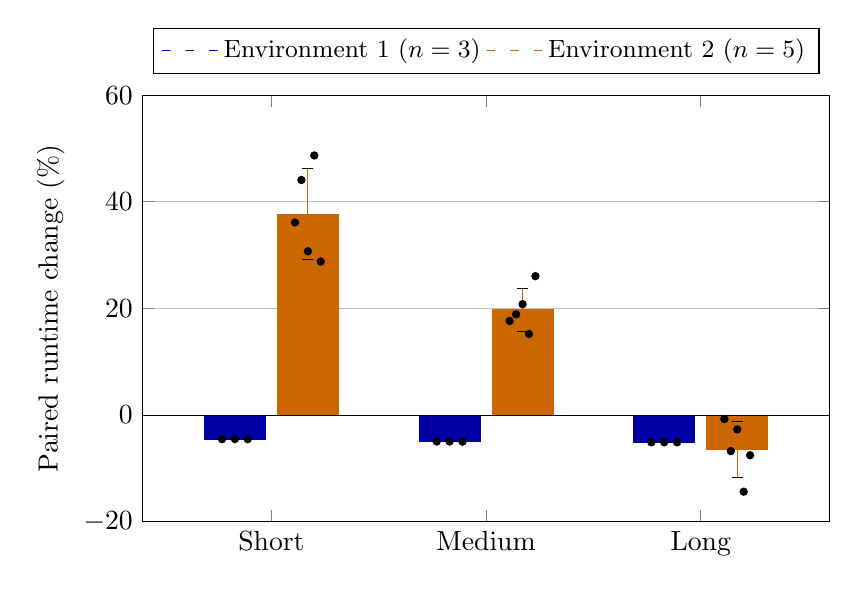
\begin{tikzpicture}\begin{axis}[width=.85\textwidth,height=7cm,xmin=-.6,xmax=2.6,ymin=-20,ymax=60,xtick={0,1,2},xticklabels={Short,Medium,Long},ylabel={Paired runtime change (\%)},legend style={at={(.5,1.05)},anchor=south,legend columns=2,font=\small},ymajorgrids=true]
\addplot[ybar,bar width=22pt,fill=blue!65!black,draw=blue!65!black,error bars/.cd,y dir=both,y explicit] coordinates {(-0.17,-4.518702515943322) +- (0,0.013983612419588681) (0.83,-4.972759574002627) +- (0,0.01531263015113631) (1.83,-5.1080291189045575) +- (0,0.0006388687927925786)};\addlegendentry{Environment 1 ($n=3$)}
\addplot[only marks,mark=*,mark size=1.3pt,black,forget plot] coordinates {(-0.23,-4.530613890120525) (-0.17,-4.503305918400253) (-0.11000000000000001,-4.522187739309188) (0.77,-4.966771331058025) (0.83,-4.961345976988894) (0.8899999999999999,-4.990161413960962) (1.77,-5.107775364024343) (1.83,-5.107556113289411) (1.8900000000000001,-5.108755879399918)};
\addplot[ybar,bar width=22pt,fill=orange!80!black,draw=orange!80!black,error bars/.cd,y dir=both,y explicit] coordinates {(0.17,37.66690998422855) +- (0,8.54813252860203) (1.17,19.713397108644475) +- (0,4.078864128468423) (2.17,-6.42312058356128) +- (0,5.256522242165112)};\addlegendentry{Environment 2 ($n=5$)}
\addplot[only marks,mark=*,mark size=1.3pt,black,forget plot] coordinates {(0.11000000000000001,36.10902959910078) (0.14,44.07596239300247) (0.17,30.693839452395775) (0.2,48.675331167208185) (0.23,28.780387309435525) (1.1099999999999999,17.63669140825637) (1.14,18.886500387722457) (1.17,20.795064347728964) (1.2,15.205769972306939) (1.23,26.042959427207634) (2.11,-0.7610558601580898) (2.14,-6.752098565253035) (2.17,-2.690881749745551) (2.1999999999999997,-14.371718841826734) (2.23,-7.539847900822994)};
\addplot[black,no marks,forget plot] coordinates {(-.6,0) (2.6,0)};\end{axis}\end{tikzpicture}\caption{V8 runtime effects by environment and run length. Bars show the mean of $100(O_i-R_i)/R_i$; whiskers show sample standard deviations, and dots show individual pairs. Negative values favor Overloaded. E1 uses Arg1=360; E2 uses Arg1=275/400/550. The groups have different workload configurations; differences must not be attributed solely to the environment.}\label{fig:v8-environments}\end{figure}\clearpage

\section{PThreads Experiments}
\label{sec:pthreads-experiments}

\subsection{Methodology}

Pthreads performance under different memory-allocation strategies is compared on a single machine using both Windows WSL and native Linux (Linux Mint, based on Ubuntu). For the general summary-statistics experiments, the matrix-size parameter, $n$, is fixed at 800 and the number of threads is fixed at 8. Each experiment performs multiplication involving 200 $n \times n$ matrices. All experiments in this section are performed on the same machine, with 16GB of RAM and an Intel i7-11370H CPU. Pthreads versions v4.0.0 and v6.0.0 are tested with either CMA v7.0.0 or regular \texttt{new} as the memory-allocation strategy. Pthreads v4.0.0 uses queues and mutexes, whereas v6.0.0 removes these mechanisms to improve cache locality and throughput at the expense of code readability and implementation simplicity.

After obtaining the summary statistics, assumption checks are performed before subsequent statistical testing. The Shapiro--Wilk test is used to evaluate normality, while Levene's test is used to evaluate equality of variances among methods. When these assumptions are reasonably satisfied, one-way ANOVA and Tukey HSD are used for inferential comparisons. ANOVA tests the null hypothesis that all method mean runtimes are equal, while Tukey HSD provides pairwise comparisons among methods while controlling the family-wise error rate. These pairwise results are then used to identify groups of methods with statistically distinguishable performance. Tukey HSD comparisons are also performed across the Linux and Windows WSL environments for corresponding methods.

A more detailed empirical scaling analysis is performed on two methods of particular interest: pthreads v4 -- CMA v7 and pthreads v6 -- regular \texttt{new}, both under native Linux. These methods are selected to examine the central trade-off of whether a simpler calculation implementation can remain competitive when paired with a custom memory allocator that improves memory-access behavior. In particular, the comparison asks whether the runtime cost of the simpler pthreads v4 implementation can be sufficiently reduced by CMA to make its increased readability and simplicity practically worthwhile.

Each method is first fit to a power-law model of the form $T(n)=cn^p$ in order to estimate its empirical scaling exponent and determine whether the two methods exhibit approximately equivalent growth rates. Each method is also fit to a full cubic polynomial. These polynomial models are used descriptively to evaluate how well cubic-shaped runtime growth represents the observed data and to investigate whether any broader runtime comparison can be supported. Because these fits are based on a finite experimental range, asymptotic extrapolations are interpreted cautiously.

\subsection{Results}

The experiments indicate that, under the appropriate execution environment, the simpler pthreads implementation can remain reasonably competitive when combined with a custom memory allocator, although it retains a runtime disadvantage relative to the highest-performing implementation.

Table~\ref{tab:pthreads-wsl-summary} presents summary statistics for the Windows WSL pthreads experiments. The results indicate a slight performance degradation when CMA v7.0.0 is used with either pthreads v4 or pthreads v6 compared with regular \texttt{new}. Table~\ref{tab:pthreads-wsl-tests} reports the Shapiro--Wilk, Levene, and one-way ANOVA results, while Tables~\ref{tab:pthreads-wsl-tukey} and~\ref{tab:pthreads-wsl-ranking} present the corresponding pairwise significance tests and performance groupings. Tukey HSD comparisons at $\alpha=0.05$ show that pthreads v6 with regular \texttt{new} has significantly lower mean runtime than all other tested methods. No statistically significant difference is found between the two memory-allocation strategies when used with pthreads v4.

The same experiments under native Linux, shown in Tables~\ref{tab:pthreads-linux-summary},~\ref{tab:pthreads-linux-tests},~\ref{tab:pthreads-linux-tukey}, and~\ref{tab:pthreads-linux-ranking}, exhibit a substantially different pattern. For pthreads v6, no statistically significant difference is found between the two memory-allocation strategies, although regular \texttt{new} has a slightly lower mean runtime. In contrast, a statistically significant difference is found between the allocation strategies for pthreads v4: using CMA v7 produces a substantially lower mean runtime than using regular \texttt{new}. The mean runtime of pthreads v4 with CMA v7 remains higher than that of pthreads v6, but the remaining performance gap may be small enough in some contexts to justify the simpler and more readable pthreads v4 implementation. These results also demonstrate that the custom allocator can substantially improve the performance of the otherwise slower implementation.

Table~\ref{tab:pthreads-linuxwindows-tukey} shows statistically significant differences for corresponding methods across the Linux and Windows WSL environments. Together with the substantially different performance groupings shown in Tables~\ref{tab:pthreads-wsl-ranking} and~\ref{tab:pthreads-linux-ranking}, these results indicate that the execution environment affects not only absolute runtime but also the relative effectiveness of the custom memory-allocation strategy.

Figure~\ref{fig:pthreads-comparison} shows runtime growth for pthreads v4 -- CMA v7 and pthreads v6 -- regular \texttt{new}. The matrix-size parameter is varied from 400 to 1800, with a single run performed for each method at each value of $n$. The pthreads v6 -- regular \texttt{new} curve exhibits very smooth growth despite the absence of repeated trials at each point, whereas pthreads v4 -- CMA v7 exhibits substantially greater size-dependent variability.

Table~\ref{tab:pthreads-runtime-fits} presents power-law and cubic-polynomial models fitted to the runtime data. The power-law fits are consistent with approximately cubic empirical scaling, with fitted exponents of 3.064 for pthreads v4 -- CMA v7 and 2.938 for pthreads v6 -- regular \texttt{new}. The regular-allocation implementation follows the fitted model particularly closely, with $R^2=0.99992$, while the CMA implementation is less regular, with $R^2=0.98632$. Full cubic-polynomial fits increase the descriptive $R^2$ values to 0.99334 and 0.99998, respectively. These results support approximately cubic growth for both methods while also showing that the CMA implementation exhibits substantially greater size-dependent variation.

Across the measured parameter values, the observed runtime ratio
$$
\frac{T_{\mathrm{CMA}}}{T_{\mathrm{regular}}}
$$
ranges from approximately 1.085 to 1.379. Thus, pthreads v4 -- CMA v7 is approximately 8.5\% to 37.9\% slower than pthreads v6 -- regular \texttt{new} over the tested range, subject to uncertainty from the use of only a single run at each parameter value. The relative disadvantage generally becomes larger at higher values of $n$, although the sequence is not monotonic.

Extrapolation beyond the measured range should be treated cautiously. The fitted power-law models have different exponents and therefore imply a runtime ratio that continues to increase with $n$. In contrast, the leading cubic terms of the polynomial fits imply an asymptotic ratio of approximately
$$
\frac{1.325\times10^{-6}}{4.232\times10^{-7}}\approx 3.13,
$$
which would correspond to CMA requiring approximately 3.13 times the runtime, or about 213\% greater runtime, in the asymptotic limit of that fitted model. These extrapolations disagree substantially and are both based on a limited finite range. Furthermore, the size-dependent variability observed for pthreads v4 -- CMA v7 suggests that its runtime may be influenced by discrete or piecewise hardware effects involving memory allocation, cache behavior, paging, alignment, or related mechanisms. Consequently, the measured runtime ratios provide a more reliable characterization of performance within the tested range than either model provides for long-range extrapolation.

\begin{table}[!t]
\centering
\caption{Windows WSL Experiments -- Summary statistics by method.}
\label{tab:pthreads-wsl-summary}
\footnotesize
\resizebox{\columnwidth}{!}{%
\begin{tabular}{lrrrr}
\toprule
Method & Mean & Std.\ Dev. & Min & Max \\
\midrule
pthreads v6.0.0 - regular new & \textbf{292.769} & 1.618 & 290.947 & 294.582 \\
pthreads v6.0.0 - CMA v7.0.0 & 300.914 & 0.627 & 299.988 & 301.544 \\
pthreads v4.0.0 - regular new & 395.795 & 3.762 & 390.184 & 400.669 \\
pthreads v4.0.0 - CMA v7.0.0 & 397.664 & 6.023 & 388.333 & 402.081 \\
\bottomrule
\end{tabular}%
}
\end{table}

\begin{table}[!t]
\centering
\caption{Windows WSL Experiments -- Shapiro--Wilk, Levene, and one-way ANOVA results.}
\label{tab:pthreads-wsl-tests}
\footnotesize
\resizebox{\columnwidth}{!}{%
\begin{tabular}{lrrl}
\toprule
Test & Test Statistic & $p$-value & Result \\
\midrule
Shapiro--Wilk & $W = 0.9111$ & 0.0668 & Normality assumption satisfied \\
Levene's test & $W = 1.1853$ & 0.3466 & Equal-variance assumption satisfied \\
One-way ANOVA & $F = 1249.0073$ & $3.560\times10^{-19}$ & Significant difference among means \\
\bottomrule
\end{tabular}%
}
\end{table}

\begin{table}[!t]
\centering
\caption{Windows WSL Experiments -- Tukey HSD pairwise comparisons ($\alpha = 0.05$).}
\label{tab:pthreads-wsl-tukey}
\footnotesize
\resizebox{\columnwidth}{!}{%
\begin{tabular}{llrl}
\toprule
Method A & Method B & $p$ & Significant \\
\midrule
pthreads v4.0.0 - regular new & pthreads v4.0.0 - CMA v7.0.0 & 0.8495 & No \\
pthreads v4.0.0 - regular new & pthreads v6.0.0 - regular new & $<0.0001$ & Yes \\
pthreads v4.0.0 - regular new & pthreads v6.0.0 - CMA v7.0.0 & $<0.0001$ & Yes \\
pthreads v4.0.0 - CMA v7.0.0 & pthreads v6.0.0 - regular new & $<0.0001$ & Yes \\
pthreads v4.0.0 - CMA v7.0.0 & pthreads v6.0.0 - CMA v7.0.0 & $<0.0001$ & Yes \\
pthreads v6.0.0 - regular new & pthreads v6.0.0 - CMA v7.0.0 & 0.0135 & Yes \\
\bottomrule
\end{tabular}%
}
\end{table}

\begin{table}[!t]
\centering
\caption{Windows WSL Experiments -- Final ranking of methods.}
\label{tab:pthreads-wsl-ranking}
\footnotesize
\resizebox{\columnwidth}{!}{%
\begin{tabular}{clrl}
\toprule
Rank & Method & Mean Time (s) & Significance Group \\
\midrule
1 & pthreads v6.0.0 - regular new & \textbf{292.769} & A \\
2 & pthreads v6.0.0 - CMA v7.0.0 & 300.914 & B \\
3 & pthreads v4.0.0 - regular new & 395.795 & C \\
4 & pthreads v4.0.0 - CMA v7.0.0 & 397.664 & C \\
\bottomrule
\end{tabular}%
}
\end{table}

\begin{table}[!t]
\centering
\caption{Linux Experiments -- Summary statistics by method.}
\label{tab:pthreads-linux-summary}
\footnotesize
\resizebox{\columnwidth}{!}{%
\begin{tabular}{lrrrr}
\toprule
Method & Mean & Std.\ Dev. & Min & Max \\
\midrule
pthreads v6.0.0 - regular new & \textbf{224.896} & 1.057 & 224.144 & 226.726 \\
pthreads v6.0.0 - CMA v7.0.0 & 226.776 & 0.843 & 225.551 & 227.932 \\
pthreads v4.0.0 - CMA v7.0.0 & 246.981 & 2.615 & 244.008 & 250.656 \\
pthreads v4.0.0 - regular new & 348.573 & 2.909 & 343.810 & 351.048 \\
\bottomrule
\end{tabular}%
}
\end{table}

\begin{table}[!t]
\centering
\caption{Linux Experiments -- Shapiro--Wilk, Levene, and one-way ANOVA results.}
\label{tab:pthreads-linux-tests}
\footnotesize
\resizebox{\columnwidth}{!}{%
\begin{tabular}{lrrl}
\toprule
Test & Test Statistic & $p$-value & Result \\
\midrule
Shapiro--Wilk & $W = 0.9627$ & 0.5985 & Normality assumption satisfied \\
Levene's test & $W = 1.5435$ & 0.2418 & Equal-variance assumption satisfied \\
One-way ANOVA & $F = 4023.3356$ & $3.148\times10^{-23}$ & Significant difference among means \\
\bottomrule
\end{tabular}%
}
\end{table}

\begin{table}[!t]
\centering
\caption{Linux Experiments -- Tukey HSD pairwise comparisons ($\alpha = 0.05$).}
\label{tab:pthreads-linux-tukey}
\footnotesize
\resizebox{\columnwidth}{!}{%
\begin{tabular}{llrl}
\toprule
Method A & Method B & $p$ & Significant \\
\midrule
pthreads v4.0.0 - regular new & pthreads v4.0.0 - CMA v7.0.0 & $<0.0001$ & Yes \\
pthreads v4.0.0 - regular new & pthreads v6.0.0 - regular new & $<0.0001$ & Yes \\
pthreads v4.0.0 - regular new & pthreads v6.0.0 - CMA v7.0.0 & $<0.0001$ & Yes \\
pthreads v4.0.0 - CMA v7.0.0 & pthreads v6.0.0 - regular new & $<0.0001$ & Yes \\
pthreads v4.0.0 - CMA v7.0.0 & pthreads v6.0.0 - CMA v7.0.0 & $<0.0001$ & Yes \\
pthreads v6.0.0 - regular new & pthreads v6.0.0 - CMA v7.0.0 & 0.4965 & No \\
\bottomrule
\end{tabular}%
}
\end{table}

\begin{table}[!t]
\centering
\caption{Linux Experiments -- Final ranking of methods.}
\label{tab:pthreads-linux-ranking}
\footnotesize
\resizebox{\columnwidth}{!}{%
\begin{tabular}{clrl}
\toprule
Rank & Method & Mean Time (s) & Significance Group \\
\midrule
1 & pthreads v6.0.0 - regular new & \textbf{224.896} & A \\
2 & pthreads v6.0.0 - CMA v7.0.0 & 226.776 & A \\
3 & pthreads v4.0.0 - CMA v7.0.0 & 246.981 & B \\
4 & pthreads v4.0.0 - regular new & 348.573 & C \\
\bottomrule
\end{tabular}%
}
\end{table}

\begin{table}[!t]
\centering
\caption{Linux vs Windows Significance Experiments -- Tukey HSD pairwise comparisons ($\alpha = 0.05$).}
\label{tab:pthreads-linuxwindows-tukey}
\footnotesize
\resizebox{\columnwidth}{!}{%
\begin{tabular}{llrl}
\toprule
Method & $p$ & Significant \\
\midrule
pthreads v4.0.0 - regular new & $<0.0001$ & Yes \\
pthreads v4.0.0 - CMA v7.0.0 & $<0.0001$ & Yes \\
pthreads v6.0.0 - regular new  & $<0.0001$ & Yes \\
pthreads v6.0.0 - CMA v7.0.0 & $<0.0001$ & Yes \\
\bottomrule
\end{tabular}%
}
\end{table}

\begin{figure}[!t]
\centering
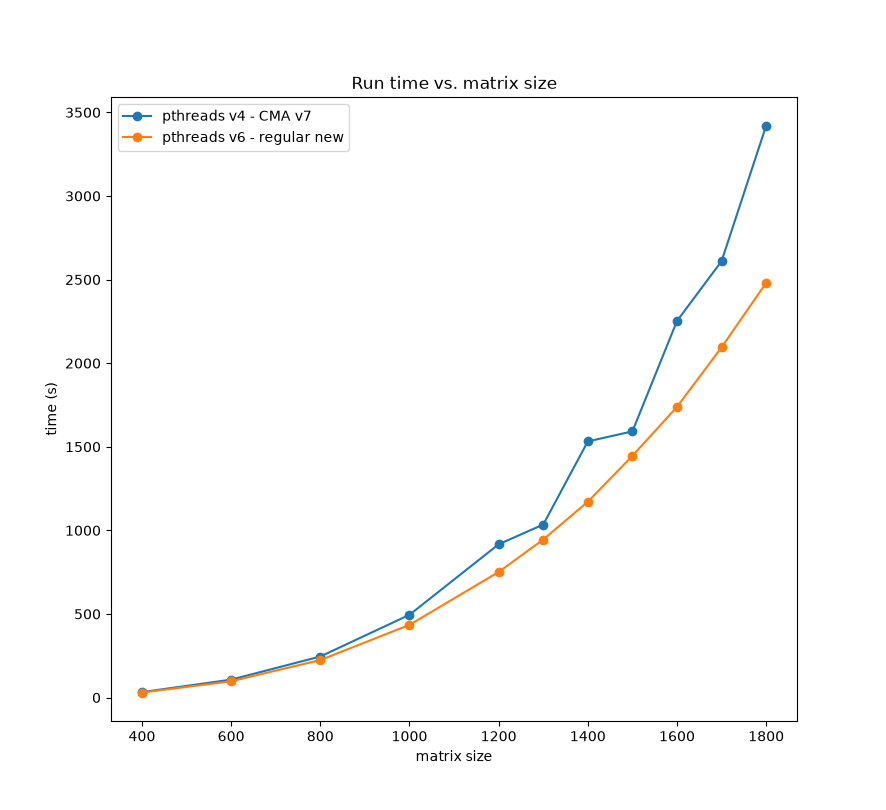
\includegraphics[width=\columnwidth]{pthreads_figure.png}
\caption{Runtime complexity comparison of pthreads v4 -- CMA v7 with pthreads v6 -- regular \texttt{new} on Linux.}
\label{fig:pthreads-comparison}
\end{figure}

\begin{table}[!t]
\centering
\caption{Empirical runtime model fits.}
\label{tab:pthreads-runtime-fits}
\footnotesize
\resizebox{\columnwidth}{!}{%
\begin{tabular}{llll}
\toprule
Method & Fit Type & Fitted Model & $R^2$ \\
\midrule
pthreads v4 -- CMA v7 & Power law & {\small $3.29\times10^{-7} n^{3.064}$} & 0.98632 \\
pthreads v6 -- regular new & Power law & {\small $6.71\times10^{-7} n^{2.938}$} & 0.99992 \\
pthreads v4 -- CMA v7 & Polynomial & {\small $1.325\times10^{-6}n^3 - 2.268\times10^{-3}n^2 + 1.912n - 478.4$} & 0.99334 \\
pthreads v6 -- regular new & Polynomial & {\small $4.232\times10^{-7}n^3 - 1.311\times10^{-5}n^2 + 3.558\times10^{-2}n - 10.07$} & 0.99998 \\
\bottomrule
\end{tabular}%
}
\end{table}

\FloatBarrier
\section{Responses to README Questions}
\label{sec:readme-questions}

The UsingMatrixClass README ends with seventeen questions.
They are grouped below into four themes: profiling and measurement, allocator
design and workload fit, hardware and operating system effects, and software
engineering practice.
Each question is quoted in italics before its response.

\subsection{Profiling and Measurement}
\label{sec:rq-measurement}

\subsubsection{Profiling Scale}
\emph{What do you notice as the profiling scale increases in each test case?}
The performance gap between the custom allocator and regular \texttt{new}
stayed roughly constant as scale increased.
Peak memory barely changed between the short, medium, and long tests.
This suggests the scale parameter repeats the same working set rather than
enlarging it, which means the pool's memory overhead stayed fixed.
Minor page faults grew almost exactly in proportion to elapsed time.
Overall, the choice of test case mattered more than the scale.

\subsubsection{Fixed Random Seed}
\emph{Why is a fixed random seed important for a fair comparison?}
It is important that all versions face the same seed to ensure fairness when
comparing performance.
This ensures that no one version is doing any more or less work than the
others.
A fixed seed also makes results reproducible.

\subsubsection{Execution Order}
\emph{How could execution order affect measured results?}
Execution order matters because each test inherits the machine state left by
whatever ran before it.
That state includes the operating system's page cache, which already holds the
executable and shared libraries after the first test has loaded them, as well
as the CPU's frequency and thermal state.
A test running second is therefore measured under different conditions than
the same test running first: whichever test runs first pays that cost and
whichever runs second gets it for free.

\subsubsection{Repeated Runs and Median Times}
\emph{Why should several runs and median times be used for profiling?}
Several runs and median times should be used for profiling to avoid the data
being skewed by outliers.
This prevents an anomaly that slowed down one run from affecting the profiling
data too much.

\subsubsection{Measurements Beyond Elapsed Time}
\emph{Which measurements should be collected in addition to elapsed time?}
Because the results are collected across multiple teams, the environment must
be recorded alongside the timing.
This includes CPU model, core count, operating system version, and compiler
version.
Additionally, each run records CPU utilization and peak memory usage.
Each run also records minor page faults, which showed that regular
\texttt{new} incurred many times more of them than the overloaded version.

\subsection{Allocator Design and Workload Fit}
\label{sec:rq-policy}

\subsubsection{Known Access Patterns and Heuristics}
\emph{When could a known access pattern make an allocator heuristic
effective?}
A heuristic is effective when the workload matches the assumption it encodes.
Knowing the pattern in advance lets you pick the heuristic that skips exactly
the work your workload would never need.

\subsubsection{System Allocator on Small Nodes}
\emph{Why might the system allocator outperform a custom allocator for small
nodes?}
Our linked-list test was the worst case for the custom allocator.
It was slower than regular \texttt{new} at every scale and had 2.55 times the
peak memory.
Our matrix-based tests differed by only 3--28\,\% in memory.
The cause is that per-allocation overhead is a fixed cost regardless of object
size, so it dominates when the objects are small.

\subsubsection{Fragmentation}
\emph{How does fragmentation affect allocation search time and memory use?}
Fragmentation means free memory exists but is split into pieces too small to
satisfy a request.
This means an allocation can fail even when total free space is
sufficient~\cite{wilson1995}.
Search time grows because there are more free-list entries to examine.

\subsubsection{Canaries and Allocation Metadata}
\emph{How do canaries and allocation metadata affect speed and memory use?}
In v7, \texttt{allocation\_overhead} is 64 bytes per allocation: a 48-byte
header, an 8-byte owner pointer, and two 4-byte canaries.
For the 72-byte linked-list node, header, alignment padding, and canaries bring
the block to 144 bytes, which the slab refill then rounds up to 192 bytes.
Every allocation writes two canaries and an owner pointer.
Every deallocation reads and compares both canaries before freeing.
This operation is cheap but can be significant when working with a small node.

\subsubsection{Cache Limits and Size Classes}
\emph{How should cache limits and size classes be selected for a workload?}
They should be chosen by measuring the workload's actual request sizes rather
than fixed in advance.
Cache limits should be sized to each thread's working set per class and capped
by a total byte budget multiplied across all threads.

\subsubsection{Workload-Specific Optimization}
\emph{When could an allocator optimized for one workload harm another
workload?}
Optimizations usually assume some specific scenario, so if that condition is
not met, the optimization can cause unnecessary overhead in another workload
compared to the ideal workload.

\subsection{Hardware and Operating System Effects}
\label{sec:rq-hardware}

\subsubsection{Matrix Calculation Time}
\emph{Why can matrix calculation time hide allocation improvements?}
Since the allocator versions do not change the matrix arithmetic, we look at
Amdahl's law~\cite{amdahl1967}.
It states that an improvement to allocation is capped by allocation's share of
total runtime.
Matrix multiplication has $O(n^3)$ arithmetic over $O(n^2)$ memory.
This means that as the matrix grows, the allocation share shrinks toward zero.

\subsubsection{Cache-Line Padding and False Sharing}
\emph{Several threads update adjacent objects. How could padding each object
to a cache-line boundary waste space yet improve performance by reducing false
sharing and cache coherence traffic?}
Cache coherence works on whole cache lines~\cite{hennessy2019}.
So, when two threads write to objects that share a line, each write
invalidates the other thread's copy and the line bounces between them.
Padding each object to a cache-line boundary wastes space, but it eliminates
that false sharing by trading cheap memory for expensive coherence traffic that
gets worse as thread count rises.

\subsection{Software Engineering Practice}
\label{sec:rq-engineering}

\subsubsection{Namespaces and Multiple Allocators}
\emph{How could namespaces support multiple allocators based on scope and
purpose?}
Namespaces let each subsystem use an allocator suited to its purpose.
Scoping allocators this way also isolates each subsystem's statistics and
failures, and a single namespace can swap a module's allocator without
changing its code.

\subsubsection{Custom Allocator Tradeoffs}
\emph{What tradeoffs come with creating and maintaining a custom allocator?}
A custom allocator can help maximize the efficiency of the program by reducing
the number of system calls and potentially memory fragmentation.
However, if the task is trivial, then the overhead from creating and
maintaining the custom allocator could slow down the entire process.
Overhead includes both runtime overhead and the overhead of writing, testing,
and maintaining the custom allocator.
The additional code can be complex and hard to read, which makes maintenance
harder than using system calls.

\subsubsection{Design, Portability, and Reusability}
\emph{Why do good design, separation of concerns, portability, and reusability
matter when code is shared across projects?}
Shared code must be readable and maintainable by people who did not write it.
This allows anyone to understand what a change will affect.
Portability was a constraint in this project because the various environments
handled the source code differently.

\subsubsection{Single Source of Truth}
\emph{Explain the importance of single source of truth in source code
management.}
A single source of truth means each piece of information is defined in exactly
one authoritative place.
This removes any ambiguity about which version is current when several people
edit the same file.

\section{Threats to Validity}
\label{sec:threats-to-validity}

The largest limitation to validity is that allocator versions were not all benchmarked on the same machine. Data were collected from Apple M3/M5 systems, several Intel systems, and Ryzen systems. The operating systems also varied, including WSL, native Linux, and macOS. CPU architectures differed as well, with some runs using ARM64 rather than the more typical x86-64. This limitation is mitigated largely by focusing on comparisons within the same environment and machine, so most experiments emphasize CMA versus regular new under otherwise matching conditions. However, when analysis crosses machine or environment boundaries, these differences cannot be fully controlled.

Another limitation is that different teams used different matrix sizes, repetition counts, linked-list sizes, and other workload parameters. Targeting specified workload-duration categories such as `short,'' `medium,'' and ``long'' also reintroduced machine- and environment-dependent variation, since achieving a similar runtime on different systems could require different workload parameters. This issue is again mitigated by keeping most analysis at the per-machine and per-environment level, but it strongly limits the ability to generalize the results into a broad characterization of expected CMA performance. Unequal numbers of repeated runs also make statistical comparisons across experiments less directly comparable and reduce statistical power in experiments with fewer observations. The typical sample size of five runs is also likely too small for assumption tests such as Shapiro--Wilk and Levene's test to provide strong evidence that their respective assumptions hold. Therefore, the more appropriate interpretation is that no violation of the tested assumption was detected, rather than that the data were conclusively shown to possess a particular distributional property.

Run-to-run observations may also not be completely independent. Repeated experiments on the same machine can inherit machine state from earlier runs, including cache state, CPU temperature, CPU frequency, memory pressure, and other operating-system state. There is also insufficient evidence that every benchmark run occurred under the same level of unrelated system activity, since the machines may have been used intermittently for other tasks. If CMA and regular-new benchmarks were repeatedly executed in a fixed order, these effects could introduce systematic bias. Even when execution order varied, uncontrolled machine state could still introduce additional noise and affect the resulting statistical analysis.

The generated executable programs may also not be fully comparable across machines because of differences in compilers, standard libraries, and toolchains, including GCC, Clang/LLVM, MSVC, MinGW, MSYS2, and related platform-specific build environments. These toolchains can differ in optimization behavior, code generation, standard-library implementation, and the underlying implementation used by regular \texttt{new}. Therefore, some measured differences between environments may reflect toolchain or runtime-library behavior in addition to allocator behavior.

The experiments do not independently measure the individual sources of runtime. Total application runtime can contain time spent on computation, allocation and deallocation, mutex contention, free-list searches, coalescing, cache hits and misses, paging, and other effects. The benchmarks primarily measure the final application-level runtime and related operating-system metrics rather than decomposing runtime into these components. As a result, explanations that attribute observed performance changes to specific allocator mechanisms should be treated as informed interpretations of the implementation and workload behavior rather than direct measurements of those mechanisms.

Finally, the results may not generalize directly to larger production or enterprise systems. The experiments were conducted on individual workstation-class machines using relatively controlled benchmark workloads. Larger systems can introduce additional factors such as higher thread counts, long-running mixed workloads, containers or virtual machines, hypervisor-level memory management, and more complex operating-system memory pressure. These layers can change allocation latency, locality, synchronization costs, paging behavior, and the relative importance of allocator overhead. Consequently, performance improvements observed in these benchmarks should be interpreted as evidence for the tested workloads and environments rather than as a guarantee of similar improvements in large-scale production deployments.
\section{Reproducibility}
\label{sec:reproducibility}

All testing scripts created by the group are included in the group's GitHub repository. The source implementations for the CMA versions and testing benchmarks are available in the course GitHub repository, with allocator versions identified by their corresponding version tags. The report also records the primary workload parameters used for the experiments, and matrix experiments include checksums that can be used to verify that reproduced executions perform the same computation and produce consistent results.

The testing scripts, source implementations, workload parameters, machine descriptions, operating-system information, and recorded experimental results together define the experimental configuration used for the reported benchmarks. The scripts automate repeated execution of the workloads and collection of profiling metrics, reducing the amount of manual intervention required to reproduce the experiments. The statistical procedures used to analyze the resulting data are also described in the report, including the significance threshold and the tests applied to the collected observations.
\section{Conclusions}
\label{sec:conclusions}

This project compared regular global \texttt{new} with overloaded global
\texttt{new} backed by eight versions of CustomMemoryAllocator.
We ran four workloads at three time scales across several machines, and we
measured elapsed time, peak memory, page faults, and context switches.

\subsection{No custom version was faster everywhere}

Version v7 lost to the system allocator in all twelve combinations of workload
and scale on the Ryzen host.
It was about 9.7 percent slower on the matrix array, 9.7 percent slower on
uniform nodes, 4.5 percent slower on nested stress, and 12 percent slower on
the linked list.
Version v6 on the Apple M3~Max did better, but only on two workloads.
It improved the matrix array by 2.3 percent and uniform nodes by 3.1 percent,
while losing 6.4 percent on nested stress and matching the system allocator on
the linked list.
In other words, the workload decided the outcome more than the allocator
version did.

\subsection{Newer versions were not better versions}

The matrix campaign ran all seven released versions on one machine with one set
of parameters.
The two simplest allocators won.
Version v1 used a single address-ordered free list with first-fit search and
finished 3.8 percent faster than the system allocator.
Version v2 was nearly identical.
From there the results got worse rather than better.
Version v5 was 2.7 percent slower than regular \texttt{new} and version v7 was
1.8 percent slower.
Each of those versions added machinery that was meant to help, such as
deferred coalescing and adaptive per-thread caches.
On this workload that machinery only added cost.

\subsection{The custom allocator traded memory for system calls}

The pool asks the operating system for memory once and never gives it back.
That choice showed up clearly in the measurements.
The overloaded programs took 97 to 99 percent fewer minor page faults than
regular \texttt{new} and spent roughly ten times less time in the kernel.
However, the savings did not cover the cost of the allocator's own
bookkeeping.
Peak memory tells the same story from the other side.
The overhead was about 4 percent on the matrix array and 3 percent on uniform
nodes, but it reached 28 percent on nested stress and 155 percent on the
linked list.

\subsection{Our improved allocator succeeded on its target and failed
elsewhere}

Version v8 started from v7 and changed the paths that matter for packed matrix
rows.
It beat regular \texttt{new} by 4.5 to 5.1 percent on the matrix array, and the
result was statistically significant at every scale.
The same changes made the linked list unusable.
Those runs had to be killed before finishing.
This is the clearest evidence in the project for the point that runs through
all of our results.
An allocator is tuned for an assumed pattern of requests, and it pays for that
assumption whenever the pattern does not hold.

\subsection{The environment mattered too}

The same v7 code was about 5 percent slower than regular \texttt{new} on
Group~1's Core i5-6400 and about 11 percent slower on our Ryzen host.
The pthreads experiments showed the same sensitivity
(\Cref{sec:pthreads-experiments}).
The custom allocator hurt performance under Windows WSL but was statistically
indistinguishable from regular \texttt{new} under native Linux.
Results from one machine should not be treated as a general claim.

\subsection{What we conclude}

A general-purpose system allocator is hard to beat because it has been tuned
for mixed workloads over decades.
A custom allocator is worth building when profiling shows that allocation is on
the critical path and the request pattern is known in advance.
Our measurements support that conclusion in both directions.
The custom versions won on the workload whose allocation pattern was regular
and predictable, and they lost badly on the workload full of small,
short-lived, irregular objects.

\section{Group Member Commitments and Contributions}
\label{sec:contributions}
Jacob Nance
- Project Manager
- Wrote automated testing script
- Profiled v2.0.0
- Cross-team ambassador
- Gathered and analyzed data from all teams
- Wrote Methodology, Statistical Results, and Charts Comparisons sections of report

% --- Appendices ---
\appendices

\section{Supporting Appendices}
\label{sec:appendices}


% --- References ---
\printbibliography

\end{document}
